% Options for packages loaded elsewhere
\PassOptionsToPackage{unicode}{hyperref}
\PassOptionsToPackage{hyphens}{url}
%
\documentclass[
]{book}
\usepackage{amsmath,amssymb}
\usepackage{iftex}
\ifPDFTeX
  \usepackage[T1]{fontenc}
  \usepackage[utf8]{inputenc}
  \usepackage{textcomp} % provide euro and other symbols
\else % if luatex or xetex
  \usepackage{unicode-math} % this also loads fontspec
  \defaultfontfeatures{Scale=MatchLowercase}
  \defaultfontfeatures[\rmfamily]{Ligatures=TeX,Scale=1}
\fi
\usepackage{lmodern}
\ifPDFTeX\else
  % xetex/luatex font selection
\fi
% Use upquote if available, for straight quotes in verbatim environments
\IfFileExists{upquote.sty}{\usepackage{upquote}}{}
\IfFileExists{microtype.sty}{% use microtype if available
  \usepackage[]{microtype}
  \UseMicrotypeSet[protrusion]{basicmath} % disable protrusion for tt fonts
}{}
\makeatletter
\@ifundefined{KOMAClassName}{% if non-KOMA class
  \IfFileExists{parskip.sty}{%
    \usepackage{parskip}
  }{% else
    \setlength{\parindent}{0pt}
    \setlength{\parskip}{6pt plus 2pt minus 1pt}}
}{% if KOMA class
  \KOMAoptions{parskip=half}}
\makeatother
\usepackage{xcolor}
\usepackage{color}
\usepackage{fancyvrb}
\newcommand{\VerbBar}{|}
\newcommand{\VERB}{\Verb[commandchars=\\\{\}]}
\DefineVerbatimEnvironment{Highlighting}{Verbatim}{commandchars=\\\{\}}
% Add ',fontsize=\small' for more characters per line
\usepackage{framed}
\definecolor{shadecolor}{RGB}{248,248,248}
\newenvironment{Shaded}{\begin{snugshade}}{\end{snugshade}}
\newcommand{\AlertTok}[1]{\textcolor[rgb]{0.94,0.16,0.16}{#1}}
\newcommand{\AnnotationTok}[1]{\textcolor[rgb]{0.56,0.35,0.01}{\textbf{\textit{#1}}}}
\newcommand{\AttributeTok}[1]{\textcolor[rgb]{0.13,0.29,0.53}{#1}}
\newcommand{\BaseNTok}[1]{\textcolor[rgb]{0.00,0.00,0.81}{#1}}
\newcommand{\BuiltInTok}[1]{#1}
\newcommand{\CharTok}[1]{\textcolor[rgb]{0.31,0.60,0.02}{#1}}
\newcommand{\CommentTok}[1]{\textcolor[rgb]{0.56,0.35,0.01}{\textit{#1}}}
\newcommand{\CommentVarTok}[1]{\textcolor[rgb]{0.56,0.35,0.01}{\textbf{\textit{#1}}}}
\newcommand{\ConstantTok}[1]{\textcolor[rgb]{0.56,0.35,0.01}{#1}}
\newcommand{\ControlFlowTok}[1]{\textcolor[rgb]{0.13,0.29,0.53}{\textbf{#1}}}
\newcommand{\DataTypeTok}[1]{\textcolor[rgb]{0.13,0.29,0.53}{#1}}
\newcommand{\DecValTok}[1]{\textcolor[rgb]{0.00,0.00,0.81}{#1}}
\newcommand{\DocumentationTok}[1]{\textcolor[rgb]{0.56,0.35,0.01}{\textbf{\textit{#1}}}}
\newcommand{\ErrorTok}[1]{\textcolor[rgb]{0.64,0.00,0.00}{\textbf{#1}}}
\newcommand{\ExtensionTok}[1]{#1}
\newcommand{\FloatTok}[1]{\textcolor[rgb]{0.00,0.00,0.81}{#1}}
\newcommand{\FunctionTok}[1]{\textcolor[rgb]{0.13,0.29,0.53}{\textbf{#1}}}
\newcommand{\ImportTok}[1]{#1}
\newcommand{\InformationTok}[1]{\textcolor[rgb]{0.56,0.35,0.01}{\textbf{\textit{#1}}}}
\newcommand{\KeywordTok}[1]{\textcolor[rgb]{0.13,0.29,0.53}{\textbf{#1}}}
\newcommand{\NormalTok}[1]{#1}
\newcommand{\OperatorTok}[1]{\textcolor[rgb]{0.81,0.36,0.00}{\textbf{#1}}}
\newcommand{\OtherTok}[1]{\textcolor[rgb]{0.56,0.35,0.01}{#1}}
\newcommand{\PreprocessorTok}[1]{\textcolor[rgb]{0.56,0.35,0.01}{\textit{#1}}}
\newcommand{\RegionMarkerTok}[1]{#1}
\newcommand{\SpecialCharTok}[1]{\textcolor[rgb]{0.81,0.36,0.00}{\textbf{#1}}}
\newcommand{\SpecialStringTok}[1]{\textcolor[rgb]{0.31,0.60,0.02}{#1}}
\newcommand{\StringTok}[1]{\textcolor[rgb]{0.31,0.60,0.02}{#1}}
\newcommand{\VariableTok}[1]{\textcolor[rgb]{0.00,0.00,0.00}{#1}}
\newcommand{\VerbatimStringTok}[1]{\textcolor[rgb]{0.31,0.60,0.02}{#1}}
\newcommand{\WarningTok}[1]{\textcolor[rgb]{0.56,0.35,0.01}{\textbf{\textit{#1}}}}
\usepackage{longtable,booktabs,array}
\usepackage{calc} % for calculating minipage widths
% Correct order of tables after \paragraph or \subparagraph
\usepackage{etoolbox}
\makeatletter
\patchcmd\longtable{\par}{\if@noskipsec\mbox{}\fi\par}{}{}
\makeatother
% Allow footnotes in longtable head/foot
\IfFileExists{footnotehyper.sty}{\usepackage{footnotehyper}}{\usepackage{footnote}}
\makesavenoteenv{longtable}
\usepackage{graphicx}
\makeatletter
\def\maxwidth{\ifdim\Gin@nat@width>\linewidth\linewidth\else\Gin@nat@width\fi}
\def\maxheight{\ifdim\Gin@nat@height>\textheight\textheight\else\Gin@nat@height\fi}
\makeatother
% Scale images if necessary, so that they will not overflow the page
% margins by default, and it is still possible to overwrite the defaults
% using explicit options in \includegraphics[width, height, ...]{}
\setkeys{Gin}{width=\maxwidth,height=\maxheight,keepaspectratio}
% Set default figure placement to htbp
\makeatletter
\def\fps@figure{htbp}
\makeatother
\setlength{\emergencystretch}{3em} % prevent overfull lines
\providecommand{\tightlist}{%
  \setlength{\itemsep}{0pt}\setlength{\parskip}{0pt}}
\setcounter{secnumdepth}{5}
\ifLuaTeX
  \usepackage{selnolig}  % disable illegal ligatures
\fi
\usepackage[]{natbib}
\bibliographystyle{apalike}
\nocite{*}
\IfFileExists{bookmark.sty}{\usepackage{bookmark}}{\usepackage{hyperref}}
\IfFileExists{xurl.sty}{\usepackage{xurl}}{} % add URL line breaks if available
\urlstyle{same}
\hypersetup{
  pdftitle={Supplemental Material for `Lexicase Selection Parameter Analysis: Varying Population Size and Test Case Redundancy with Diagnostic Metrics'},
  pdfauthor={Jose Guadalupe Hernandez, Anil Kumar Saini, Jason H. Moore},
  hidelinks,
  pdfcreator={LaTeX via pandoc}}

\title{Supplemental Material for `Lexicase Selection Parameter Analysis: Varying Population Size and Test Case Redundancy with Diagnostic Metrics'}
\author{Jose Guadalupe Hernandez, Anil Kumar Saini, Jason H. Moore}
\date{2024-07-24}

\begin{document}
\maketitle

{
\setcounter{tocdepth}{1}
\tableofcontents
}
\begin{Shaded}
\begin{Highlighting}[]
\FunctionTok{library}\NormalTok{(ggplot2)}
\FunctionTok{library}\NormalTok{(cowplot)}
\FunctionTok{library}\NormalTok{(dplyr)}
\FunctionTok{library}\NormalTok{(PupillometryR)}
\FunctionTok{library}\NormalTok{(scales) }\CommentTok{\# to access break formatting functions}


\NormalTok{NAMES }\OtherTok{=} \FunctionTok{c}\NormalTok{(}\DecValTok{50}\NormalTok{,}\DecValTok{100}\NormalTok{,}\DecValTok{500}\NormalTok{,}\DecValTok{1000}\NormalTok{,}\DecValTok{5000}\NormalTok{)}
\NormalTok{SHAPE }\OtherTok{\textless{}{-}} \FunctionTok{c}\NormalTok{(}\DecValTok{25}\NormalTok{,}\DecValTok{21}\NormalTok{,}\DecValTok{22}\NormalTok{,}\DecValTok{23}\NormalTok{,}\DecValTok{24}\NormalTok{)}
\NormalTok{cb\_palette }\OtherTok{\textless{}{-}} \FunctionTok{c}\NormalTok{(}\StringTok{\textquotesingle{}\#648FFF\textquotesingle{}}\NormalTok{,}\StringTok{\textquotesingle{}\#FE6100\textquotesingle{}}\NormalTok{,}\StringTok{\textquotesingle{}\#DC267F\textquotesingle{}}\NormalTok{,}\StringTok{\textquotesingle{}\#785EF0\textquotesingle{}}\NormalTok{,}\StringTok{\textquotesingle{}\#FFB000\textquotesingle{}}\NormalTok{)}
\NormalTok{TSIZE }\OtherTok{\textless{}{-}} \DecValTok{16}

\NormalTok{p\_theme }\OtherTok{\textless{}{-}} \FunctionTok{theme}\NormalTok{(}
  \AttributeTok{plot.title =} \FunctionTok{element\_text}\NormalTok{( }\AttributeTok{face =} \StringTok{"bold"}\NormalTok{, }\AttributeTok{size =} \DecValTok{16}\NormalTok{, }\AttributeTok{hjust=}\FloatTok{0.5}\NormalTok{),}
  \AttributeTok{panel.border =} \FunctionTok{element\_blank}\NormalTok{(),}
  \AttributeTok{panel.grid.minor =} \FunctionTok{element\_blank}\NormalTok{(),}
  \AttributeTok{legend.title=}\FunctionTok{element\_text}\NormalTok{(}\AttributeTok{size=}\DecValTok{16}\NormalTok{),}
  \AttributeTok{legend.text=}\FunctionTok{element\_text}\NormalTok{(}\AttributeTok{size=}\DecValTok{16}\NormalTok{),}
  \AttributeTok{axis.title =} \FunctionTok{element\_text}\NormalTok{(}\AttributeTok{size=}\DecValTok{16}\NormalTok{),}
  \AttributeTok{axis.text =} \FunctionTok{element\_text}\NormalTok{(}\AttributeTok{size=}\DecValTok{16}\NormalTok{),}
  \AttributeTok{legend.position=}\StringTok{"bottom"}\NormalTok{,}
  \AttributeTok{panel.background =} \FunctionTok{element\_rect}\NormalTok{(}\AttributeTok{fill =} \StringTok{"\#f1f2f5"}\NormalTok{,}
                                  \AttributeTok{colour =} \StringTok{"white"}\NormalTok{,}
                                  \AttributeTok{size =} \FloatTok{0.5}\NormalTok{, }\AttributeTok{linetype =} \StringTok{"solid"}\NormalTok{)}
\NormalTok{)}
\end{Highlighting}
\end{Shaded}

\hypertarget{introduction}{%
\chapter{Introduction}\label{introduction}}

This is not intended as a stand-alone document, but as a companion to our manuscript.

\hypertarget{about-our-supplemental-material}{%
\section{About our supplemental material}\label{about-our-supplemental-material}}

As you may have noticed (unless you're reading a pdf version of this), our supplemental material is hosted using \href{https://pages.github.com/}{GitHub pages}.
We compiled our data analyses and supplemental documentation into this nifty web-accessible book using \href{https://bookdown.org}{bookdown}.

The code used for this supplemental material can be found in \href{https://github.com/jgh9094/GPTP-2024-Lexicase-Analysis}{this GitHub repository}.

Our supplemental material includes the following:

\begin{itemize}
\tightlist
\item
  Exploitation rate results (Section \ref{exploitation-rate-results})
\item
  Standard contradictory rates results (Section \ref{contradictory-objectives-100-results})
\item
  Contradictory rates results w/ 100 redundant test cases (Section \ref{contradictory-objectives-200-results})
\item
  Contradictory rates results w/ 200 redundant test cases (Section \ref{contradictory-objectives-300-results})
\item
  Contradictory rates results w/ 400 redundant test cases (Section \ref{contradictory-objectives-500-results})
\end{itemize}

\hypertarget{contributing-authors}{%
\section{Contributing authors}\label{contributing-authors}}

\begin{itemize}
\tightlist
\item
  \href{https://jgh9094.github.io/}{Jose Guadalupe Hernandez}
\item
  \href{https://theaksaini.github.io/}{Anil Kumar Saini}
\item
  \href{https://jasonhmoore.org/}{Jason H. Moore}
\end{itemize}

\hypertarget{exploitation-rate-results}{%
\chapter{Exploitation rate results}\label{exploitation-rate-results}}

Here we report the \textbf{performance} and evaluation a \textbf{satisfactory solution} was found on the exploitation rate diagnostic.
50 replicates were conducted for each population size explored.
Performance is defined at the average trait performance, where we collect the best performing solution in each generation over time and the best performing solution evolved.
A satisfactory solution is defined as a solution that has a phenotype with all traits greater than or equal to 99.0.

\hypertarget{analysis-setup}{%
\section{Analysis setup}\label{analysis-setup}}

\begin{Shaded}
\begin{Highlighting}[]
\FunctionTok{library}\NormalTok{(ggplot2)}
\FunctionTok{library}\NormalTok{(cowplot)}
\FunctionTok{library}\NormalTok{(dplyr)}
\FunctionTok{library}\NormalTok{(PupillometryR)}

\CommentTok{\# over time data }
\NormalTok{over\_time }\OtherTok{\textless{}{-}} \FunctionTok{read.csv}\NormalTok{(}\StringTok{"../Paper\_Data/Exploitation/ot.csv"}\NormalTok{, }\AttributeTok{header =} \ConstantTok{TRUE}\NormalTok{, }\AttributeTok{stringsAsFactors =} \ConstantTok{FALSE}\NormalTok{)}
\NormalTok{over\_time}\SpecialCharTok{$}\NormalTok{pop\_size }\OtherTok{\textless{}{-}} \FunctionTok{factor}\NormalTok{(over\_time}\SpecialCharTok{$}\NormalTok{pop\_size, }\AttributeTok{levels =}\NormalTok{ NAMES)}

\CommentTok{\# best performance data}
\NormalTok{best }\OtherTok{\textless{}{-}} \FunctionTok{read.csv}\NormalTok{(}\StringTok{\textquotesingle{}../Paper\_Data/Exploitation/best.csv\textquotesingle{}}\NormalTok{, }\AttributeTok{header =} \ConstantTok{TRUE}\NormalTok{, }\AttributeTok{stringsAsFactors =} \ConstantTok{FALSE}\NormalTok{)}
\NormalTok{best}\SpecialCharTok{$}\NormalTok{pop\_size }\OtherTok{\textless{}{-}} \FunctionTok{factor}\NormalTok{(best}\SpecialCharTok{$}\NormalTok{pop\_size, }\AttributeTok{levels =}\NormalTok{ NAMES)}

\CommentTok{\# get the data}
\NormalTok{ssf }\OtherTok{\textless{}{-}} \FunctionTok{read.csv}\NormalTok{(}\StringTok{\textquotesingle{}../Paper\_Data/Exploitation/ssf.csv\textquotesingle{}}\NormalTok{, }\AttributeTok{header =} \ConstantTok{TRUE}\NormalTok{, }\AttributeTok{stringsAsFactors =} \ConstantTok{FALSE}\NormalTok{)}
\NormalTok{ssf}\SpecialCharTok{$}\NormalTok{pop\_size }\OtherTok{\textless{}{-}} \FunctionTok{factor}\NormalTok{(ssf}\SpecialCharTok{$}\NormalTok{pop\_size, }\AttributeTok{levels =}\NormalTok{ NAMES)}
\NormalTok{ssf }\OtherTok{\textless{}{-}} \FunctionTok{filter}\NormalTok{(ssf, evaluation }\SpecialCharTok{\textless{}=} \FloatTok{1.5}\SpecialCharTok{*}\DecValTok{10}\SpecialCharTok{\^{}}\DecValTok{9}\NormalTok{)}
\end{Highlighting}
\end{Shaded}

\hypertarget{performance-over-time}{%
\section{Performance over time}\label{performance-over-time}}

Performance of the best solution in the population at each generation over time.

\begin{Shaded}
\begin{Highlighting}[]
\CommentTok{\# aggregate }
\NormalTok{lines }\OtherTok{=}\NormalTok{ over\_time }\SpecialCharTok{\%\textgreater{}\%}
  \FunctionTok{group\_by}\NormalTok{(pop\_size, eval) }\SpecialCharTok{\%\textgreater{}\%}
\NormalTok{  dplyr}\SpecialCharTok{::}\FunctionTok{summarise}\NormalTok{(}
    \AttributeTok{min =} \FunctionTok{min}\NormalTok{(performance),}
    \AttributeTok{mean =} \FunctionTok{mean}\NormalTok{(performance),}
    \AttributeTok{max =} \FunctionTok{max}\NormalTok{(performance)}
\NormalTok{  )}
\NormalTok{lines}\SpecialCharTok{$}\NormalTok{pop\_size }\OtherTok{\textless{}{-}} \FunctionTok{factor}\NormalTok{(lines}\SpecialCharTok{$}\NormalTok{pop\_size, }\AttributeTok{levels =}\NormalTok{ NAMES)}

\FunctionTok{ggplot}\NormalTok{(lines, }\FunctionTok{aes}\NormalTok{(}\AttributeTok{x=}\NormalTok{eval, }\AttributeTok{y=}\NormalTok{mean, }\AttributeTok{group =}\NormalTok{ pop\_size, }\AttributeTok{fill =}\NormalTok{ pop\_size, }\AttributeTok{color =}\NormalTok{ pop\_size, }\AttributeTok{shape =}\NormalTok{ pop\_size)) }\SpecialCharTok{+}
  \FunctionTok{geom\_ribbon}\NormalTok{(}\FunctionTok{aes}\NormalTok{(}\AttributeTok{ymin =}\NormalTok{ min, }\AttributeTok{ymax =}\NormalTok{ max), }\AttributeTok{alpha =} \FloatTok{0.1}\NormalTok{) }\SpecialCharTok{+}
  \FunctionTok{geom\_line}\NormalTok{(}\AttributeTok{linewidth =} \FloatTok{0.5}\NormalTok{) }\SpecialCharTok{+}
  \FunctionTok{geom\_point}\NormalTok{(}\AttributeTok{data =} \FunctionTok{filter}\NormalTok{(lines, eval }\SpecialCharTok{\%\%} \DecValTok{100000000} \SpecialCharTok{==} \DecValTok{0} \SpecialCharTok{\&}\NormalTok{ eval }\SpecialCharTok{!=} \DecValTok{0}\NormalTok{), }\AttributeTok{size =} \FloatTok{1.0}\NormalTok{, }\AttributeTok{stroke =} \FloatTok{2.0}\NormalTok{, }\AttributeTok{alpha =} \FloatTok{1.0}\NormalTok{) }\SpecialCharTok{+}
  \FunctionTok{scale\_y\_continuous}\NormalTok{(}
    \AttributeTok{name=}\StringTok{"Average trait score"}\NormalTok{,}
    \AttributeTok{limits=}\FunctionTok{c}\NormalTok{(}\DecValTok{0}\NormalTok{, }\DecValTok{100}\NormalTok{),}
    \AttributeTok{breaks=}\FunctionTok{seq}\NormalTok{(}\DecValTok{0}\NormalTok{,}\DecValTok{100}\NormalTok{, }\DecValTok{25}\NormalTok{),}
    \AttributeTok{labels=}\FunctionTok{c}\NormalTok{(}\StringTok{"0"}\NormalTok{, }\StringTok{"25"}\NormalTok{, }\StringTok{"50"}\NormalTok{, }\StringTok{"75"}\NormalTok{, }\StringTok{"100"}\NormalTok{)}
\NormalTok{  ) }\SpecialCharTok{+}
  \FunctionTok{scale\_x\_continuous}\NormalTok{(}
    \AttributeTok{name=}\StringTok{"Evaluation"}\NormalTok{,}
    \AttributeTok{labels =} \FunctionTok{c}\NormalTok{(}\StringTok{\textquotesingle{}0.0e+0\textquotesingle{}}\NormalTok{, }\StringTok{\textquotesingle{}5.0e+8\textquotesingle{}}\NormalTok{,}\StringTok{\textquotesingle{}1.0e+9\textquotesingle{}}\NormalTok{,}\StringTok{\textquotesingle{}1.5e+9\textquotesingle{}}\NormalTok{),}
    \AttributeTok{limits =} \FunctionTok{c}\NormalTok{(}\DecValTok{0}\NormalTok{,}\DecValTok{1520000000}\NormalTok{)}
    
\NormalTok{  ) }\SpecialCharTok{+}
  \FunctionTok{scale\_shape\_manual}\NormalTok{(}\AttributeTok{values=}\NormalTok{SHAPE)}\SpecialCharTok{+}
  \FunctionTok{scale\_colour\_manual}\NormalTok{(}\AttributeTok{values =}\NormalTok{ cb\_palette) }\SpecialCharTok{+}
  \FunctionTok{scale\_fill\_manual}\NormalTok{(}\AttributeTok{values =}\NormalTok{ cb\_palette) }\SpecialCharTok{+}
  \FunctionTok{ggtitle}\NormalTok{(}\StringTok{\textquotesingle{}Performance over time\textquotesingle{}}\NormalTok{)}\SpecialCharTok{+}
\NormalTok{  p\_theme }\SpecialCharTok{+}
  \FunctionTok{guides}\NormalTok{(}
    \AttributeTok{shape=}\FunctionTok{guide\_legend}\NormalTok{(}\AttributeTok{nrow=}\DecValTok{2}\NormalTok{, }\AttributeTok{title.position =} \StringTok{"left"}\NormalTok{, }\AttributeTok{title =} \StringTok{\textquotesingle{}Population}\SpecialCharTok{\textbackslash{}n}\StringTok{Size\textquotesingle{}}\NormalTok{),}
    \AttributeTok{color=}\FunctionTok{guide\_legend}\NormalTok{(}\AttributeTok{nrow=}\DecValTok{2}\NormalTok{, }\AttributeTok{title.position =} \StringTok{"left"}\NormalTok{, }\AttributeTok{title =} \StringTok{\textquotesingle{}Population}\SpecialCharTok{\textbackslash{}n}\StringTok{Size\textquotesingle{}}\NormalTok{),}
    \AttributeTok{fill=}\FunctionTok{guide\_legend}\NormalTok{(}\AttributeTok{nrow=}\DecValTok{2}\NormalTok{, }\AttributeTok{title.position =} \StringTok{"left"}\NormalTok{, }\AttributeTok{title =} \StringTok{\textquotesingle{}Population}\SpecialCharTok{\textbackslash{}n}\StringTok{Size\textquotesingle{}}\NormalTok{)}
\NormalTok{  )}
\end{Highlighting}
\end{Shaded}

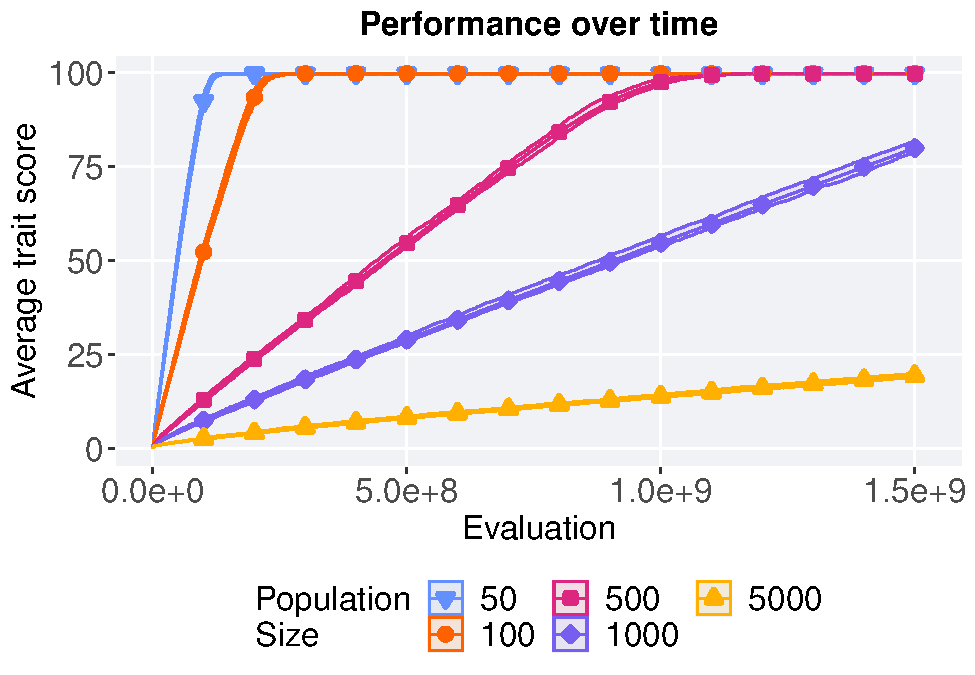
\includegraphics[width=1\linewidth]{lexicase-analysis-supplemental_files/figure-latex/exp-perf-ot-1}

\hypertarget{best-performance-evolved}{%
\section{Best performance evolved}\label{best-performance-evolved}}

Performance of the best solution found throughout the entire evolutionary run.

\begin{Shaded}
\begin{Highlighting}[]
\FunctionTok{ggplot}\NormalTok{(best, }\FunctionTok{aes}\NormalTok{(}\AttributeTok{x =}\NormalTok{ pop\_size, }\AttributeTok{y =}\NormalTok{ performance, }\AttributeTok{color =}\NormalTok{ pop\_size, }\AttributeTok{fill =}\NormalTok{ pop\_size, }\AttributeTok{shape =}\NormalTok{ pop\_size)) }\SpecialCharTok{+}
  \FunctionTok{geom\_flat\_violin}\NormalTok{(}\AttributeTok{position =} \FunctionTok{position\_nudge}\NormalTok{(}\AttributeTok{x =}\NormalTok{ .}\DecValTok{1}\NormalTok{, }\AttributeTok{y =} \DecValTok{0}\NormalTok{), }\AttributeTok{scale =} \StringTok{\textquotesingle{}width\textquotesingle{}}\NormalTok{, }\AttributeTok{alpha =} \FloatTok{0.2}\NormalTok{, }\AttributeTok{width =} \FloatTok{1.5}\NormalTok{) }\SpecialCharTok{+}
  \FunctionTok{geom\_boxplot}\NormalTok{(}\AttributeTok{color =} \StringTok{\textquotesingle{}black\textquotesingle{}}\NormalTok{, }\AttributeTok{width =}\NormalTok{ .}\DecValTok{07}\NormalTok{, }\AttributeTok{outlier.shape =} \ConstantTok{NA}\NormalTok{, }\AttributeTok{alpha =} \FloatTok{0.0}\NormalTok{, }\AttributeTok{size =} \FloatTok{1.0}\NormalTok{, }\AttributeTok{position =} \FunctionTok{position\_nudge}\NormalTok{(}\AttributeTok{x =}\NormalTok{ .}\DecValTok{16}\NormalTok{, }\AttributeTok{y =} \DecValTok{0}\NormalTok{)) }\SpecialCharTok{+}
  \FunctionTok{geom\_point}\NormalTok{(}\AttributeTok{position =} \FunctionTok{position\_jitter}\NormalTok{(}\AttributeTok{width =} \FloatTok{0.02}\NormalTok{, }\AttributeTok{height =} \FloatTok{0.0001}\NormalTok{), }\AttributeTok{size =} \FloatTok{1.5}\NormalTok{, }\AttributeTok{alpha =} \FloatTok{1.0}\NormalTok{) }\SpecialCharTok{+}
  \FunctionTok{scale\_y\_continuous}\NormalTok{(}
    \AttributeTok{name=}\StringTok{"Average trait score"}\NormalTok{,}
    \AttributeTok{limits=}\FunctionTok{c}\NormalTok{(}\DecValTok{0}\NormalTok{, }\DecValTok{100}\NormalTok{),}
    \AttributeTok{breaks=}\FunctionTok{seq}\NormalTok{(}\DecValTok{0}\NormalTok{,}\DecValTok{100}\NormalTok{, }\DecValTok{25}\NormalTok{),}
    \AttributeTok{labels=}\FunctionTok{c}\NormalTok{(}\StringTok{"0"}\NormalTok{, }\StringTok{"25"}\NormalTok{, }\StringTok{"50"}\NormalTok{, }\StringTok{"75"}\NormalTok{, }\StringTok{"100"}\NormalTok{)}
\NormalTok{  ) }\SpecialCharTok{+}
  \FunctionTok{scale\_x\_discrete}\NormalTok{(}
    \AttributeTok{name=}\StringTok{"Population Size"}
\NormalTok{  )}\SpecialCharTok{+}
  \FunctionTok{scale\_shape\_manual}\NormalTok{(}\AttributeTok{values=}\NormalTok{SHAPE)}\SpecialCharTok{+}
  \FunctionTok{scale\_colour\_manual}\NormalTok{(}\AttributeTok{values =}\NormalTok{ cb\_palette, ) }\SpecialCharTok{+}
  \FunctionTok{scale\_fill\_manual}\NormalTok{(}\AttributeTok{values =}\NormalTok{ cb\_palette) }\SpecialCharTok{+}
  \FunctionTok{ggtitle}\NormalTok{(}\StringTok{\textquotesingle{}Best performance throughout\textquotesingle{}}\NormalTok{)}\SpecialCharTok{+}
\NormalTok{  p\_theme}\SpecialCharTok{+} \FunctionTok{coord\_flip}\NormalTok{() }\SpecialCharTok{+}
  \FunctionTok{guides}\NormalTok{(}
    \AttributeTok{shape=}\FunctionTok{guide\_legend}\NormalTok{(}\AttributeTok{nrow=}\DecValTok{2}\NormalTok{, }\AttributeTok{title.position =} \StringTok{"left"}\NormalTok{, }\AttributeTok{title =} \StringTok{\textquotesingle{}Population}\SpecialCharTok{\textbackslash{}n}\StringTok{Size\textquotesingle{}}\NormalTok{),}
    \AttributeTok{color=}\FunctionTok{guide\_legend}\NormalTok{(}\AttributeTok{nrow=}\DecValTok{2}\NormalTok{, }\AttributeTok{title.position =} \StringTok{"left"}\NormalTok{, }\AttributeTok{title =} \StringTok{\textquotesingle{}Population}\SpecialCharTok{\textbackslash{}n}\StringTok{Size\textquotesingle{}}\NormalTok{),}
    \AttributeTok{fill=}\FunctionTok{guide\_legend}\NormalTok{(}\AttributeTok{nrow=}\DecValTok{2}\NormalTok{, }\AttributeTok{title.position =} \StringTok{"left"}\NormalTok{, }\AttributeTok{title =} \StringTok{\textquotesingle{}Population}\SpecialCharTok{\textbackslash{}n}\StringTok{Size\textquotesingle{}}\NormalTok{)}
\NormalTok{  )}
\end{Highlighting}
\end{Shaded}

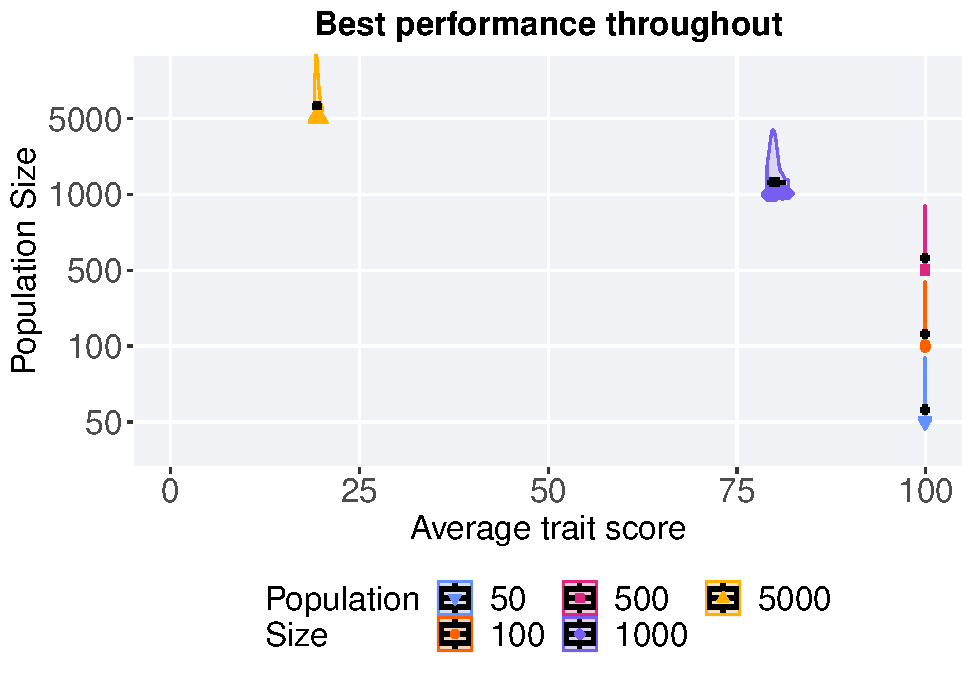
\includegraphics[width=1\linewidth]{lexicase-analysis-supplemental_files/figure-latex/exp-perf-best-1}

\hypertarget{summary-statistics}{%
\subsection{Summary statistics}\label{summary-statistics}}

\begin{Shaded}
\begin{Highlighting}[]
\NormalTok{best }\SpecialCharTok{\%\textgreater{}\%}
  \FunctionTok{group\_by}\NormalTok{(pop\_size) }\SpecialCharTok{\%\textgreater{}\%}
\NormalTok{  dplyr}\SpecialCharTok{::}\FunctionTok{summarise}\NormalTok{(}
    \AttributeTok{count =} \FunctionTok{n}\NormalTok{(),}
    \AttributeTok{na\_cnt =} \FunctionTok{sum}\NormalTok{(}\FunctionTok{is.na}\NormalTok{(performance)),}
    \AttributeTok{min =} \FunctionTok{min}\NormalTok{(performance, }\AttributeTok{na.rm =} \ConstantTok{TRUE}\NormalTok{),}
    \AttributeTok{median =} \FunctionTok{median}\NormalTok{(performance, }\AttributeTok{na.rm =} \ConstantTok{TRUE}\NormalTok{),}
    \AttributeTok{mean =} \FunctionTok{mean}\NormalTok{(performance, }\AttributeTok{na.rm =} \ConstantTok{TRUE}\NormalTok{),}
    \AttributeTok{max =} \FunctionTok{max}\NormalTok{(performance, }\AttributeTok{na.rm =} \ConstantTok{TRUE}\NormalTok{),}
    \AttributeTok{IQR =} \FunctionTok{IQR}\NormalTok{(performance, }\AttributeTok{na.rm =} \ConstantTok{TRUE}\NormalTok{)}
\NormalTok{  )}
\end{Highlighting}
\end{Shaded}

\begin{verbatim}
## # A tibble: 5 x 8
##   pop_size count na_cnt   min median  mean   max    IQR
##   <fct>    <int>  <int> <dbl>  <dbl> <dbl> <dbl>  <dbl>
## 1 50          50      0  99.9   99.9  99.9  99.9 0.0149
## 2 100         50      0  99.9   99.9  99.9  99.9 0.0166
## 3 500         50      0  99.9   99.9  99.9  99.9 0.0235
## 4 1000        50      0  79.0   79.9  80.0  81.8 0.779 
## 5 5000        50      0  19.0   19.4  19.4  20.0 0.299
\end{verbatim}

\hypertarget{kruskal-wallis-test}{%
\subsection{Kruskal-Wallis test}\label{kruskal-wallis-test}}

\begin{Shaded}
\begin{Highlighting}[]
\FunctionTok{kruskal.test}\NormalTok{(performance }\SpecialCharTok{\textasciitilde{}}\NormalTok{ pop\_size, }\AttributeTok{data =}\NormalTok{ best)}
\end{Highlighting}
\end{Shaded}

\begin{verbatim}
## 
##  Kruskal-Wallis rank sum test
## 
## data:  performance by pop_size
## Kruskal-Wallis chi-squared = 198.29, df = 4, p-value < 2.2e-16
\end{verbatim}

\hypertarget{pairwise-wilcoxon-test}{%
\subsection{Pairwise wilcoxon test}\label{pairwise-wilcoxon-test}}

\begin{Shaded}
\begin{Highlighting}[]
\FunctionTok{pairwise.wilcox.test}\NormalTok{(}\AttributeTok{x =}\NormalTok{ best}\SpecialCharTok{$}\NormalTok{performance, }\AttributeTok{g =}\NormalTok{ best}\SpecialCharTok{$}\NormalTok{pop\_size, }\AttributeTok{p.adjust.method =} \StringTok{"bonferroni"}\NormalTok{,}
                     \AttributeTok{paired =} \ConstantTok{FALSE}\NormalTok{, }\AttributeTok{conf.int =} \ConstantTok{FALSE}\NormalTok{, }\AttributeTok{alternative =} \StringTok{\textquotesingle{}l\textquotesingle{}}\NormalTok{)}
\end{Highlighting}
\end{Shaded}

\begin{verbatim}
## 
##  Pairwise comparisons using Wilcoxon rank sum test with continuity correction 
## 
## data:  best$performance and best$pop_size 
## 
##      50      100     500     1000   
## 100  1.00000 -       -       -      
## 500  0.00078 0.00059 -       -      
## 1000 < 2e-16 < 2e-16 < 2e-16 -      
## 5000 < 2e-16 < 2e-16 < 2e-16 < 2e-16
## 
## P value adjustment method: bonferroni
\end{verbatim}

\hypertarget{evaluation-satisfactory-solution-if-found}{%
\section{Evaluation satisfactory solution if found}\label{evaluation-satisfactory-solution-if-found}}

Evaluation a satisfactory solution is found for each population size.

\begin{Shaded}
\begin{Highlighting}[]
\FunctionTok{ggplot}\NormalTok{(ssf, }\FunctionTok{aes}\NormalTok{(}\AttributeTok{x =}\NormalTok{ pop\_size, }\AttributeTok{y =}\NormalTok{ evaluation, }\AttributeTok{color =}\NormalTok{ pop\_size, }\AttributeTok{fill =}\NormalTok{ pop\_size, }\AttributeTok{shape =}\NormalTok{ pop\_size)) }\SpecialCharTok{+}
  \FunctionTok{geom\_flat\_violin}\NormalTok{(}\AttributeTok{position =} \FunctionTok{position\_nudge}\NormalTok{(}\AttributeTok{x =} \FloatTok{0.12}\NormalTok{, }\AttributeTok{y =} \DecValTok{0}\NormalTok{), }\AttributeTok{scale =} \StringTok{\textquotesingle{}width\textquotesingle{}}\NormalTok{, }\AttributeTok{alpha =} \FloatTok{0.2}\NormalTok{, }\AttributeTok{width =} \FloatTok{1.5}\NormalTok{) }\SpecialCharTok{+}
  \FunctionTok{geom\_boxplot}\NormalTok{(}\AttributeTok{color =} \StringTok{\textquotesingle{}black\textquotesingle{}}\NormalTok{, }\AttributeTok{width =}\NormalTok{ .}\DecValTok{08}\NormalTok{, }\AttributeTok{outlier.shape =} \ConstantTok{NA}\NormalTok{, }\AttributeTok{alpha =} \FloatTok{0.0}\NormalTok{, }\AttributeTok{size =} \FloatTok{0.8}\NormalTok{, }\AttributeTok{position =} \FunctionTok{position\_nudge}\NormalTok{(}\AttributeTok{x =}\NormalTok{ .}\DecValTok{19}\NormalTok{, }\AttributeTok{y =} \DecValTok{0}\NormalTok{)) }\SpecialCharTok{+}
  \FunctionTok{geom\_point}\NormalTok{(}\AttributeTok{position =} \FunctionTok{position\_jitter}\NormalTok{(}\AttributeTok{width =} \FloatTok{0.03}\NormalTok{, }\AttributeTok{height =} \FloatTok{0.000001}\NormalTok{), }\AttributeTok{size =} \FloatTok{1.5}\NormalTok{, }\AttributeTok{alpha =} \FloatTok{1.0}\NormalTok{) }\SpecialCharTok{+}
  \FunctionTok{scale\_y\_continuous}\NormalTok{(}
    \AttributeTok{name =} \StringTok{\textquotesingle{}Evaluation\textquotesingle{}}\NormalTok{,}
    \AttributeTok{breaks =} \FunctionTok{c}\NormalTok{(}\DecValTok{100000000}\NormalTok{,}\DecValTok{500000000}\NormalTok{,}\DecValTok{1000000000}\NormalTok{,}\DecValTok{1500000000}\NormalTok{),}
    \AttributeTok{labels =} \FunctionTok{c}\NormalTok{(}\StringTok{\textquotesingle{}1.0e+8\textquotesingle{}}\NormalTok{, }\StringTok{\textquotesingle{}5.0e+8\textquotesingle{}}\NormalTok{,}\StringTok{\textquotesingle{}1.0e+9\textquotesingle{}}\NormalTok{,}\StringTok{\textquotesingle{}1.5e+9\textquotesingle{}}\NormalTok{),}
    \AttributeTok{limits =} \FunctionTok{c}\NormalTok{(}\DecValTok{100000000}\NormalTok{,}\DecValTok{1500000000}\NormalTok{)}
\NormalTok{    ) }\SpecialCharTok{+}
  \FunctionTok{scale\_x\_discrete}\NormalTok{(}
    \AttributeTok{name=}\StringTok{"Population Size"}\NormalTok{,}
\NormalTok{  )}\SpecialCharTok{+}
  \FunctionTok{scale\_shape\_manual}\NormalTok{(}\AttributeTok{values=}\NormalTok{SHAPE, )}\SpecialCharTok{+}
  \FunctionTok{scale\_colour\_manual}\NormalTok{(}\AttributeTok{values =}\NormalTok{ cb\_palette, ) }\SpecialCharTok{+}
  \FunctionTok{scale\_fill\_manual}\NormalTok{(}\AttributeTok{values =}\NormalTok{ cb\_palette) }\SpecialCharTok{+}
  \FunctionTok{ggtitle}\NormalTok{(}\FunctionTok{bquote}\NormalTok{(}\StringTok{\textquotesingle{}Evaluation Satisfactory Solution Found\textquotesingle{}}\NormalTok{))}\SpecialCharTok{+}
\NormalTok{  p\_theme }\SpecialCharTok{+} \FunctionTok{coord\_flip}\NormalTok{() }\SpecialCharTok{+}
  \FunctionTok{guides}\NormalTok{(}
    \AttributeTok{shape=}\FunctionTok{guide\_legend}\NormalTok{(}\AttributeTok{nrow=}\DecValTok{2}\NormalTok{, }\AttributeTok{title.position =} \StringTok{"left"}\NormalTok{, }\AttributeTok{title =} \StringTok{\textquotesingle{}Population}\SpecialCharTok{\textbackslash{}n}\StringTok{Size\textquotesingle{}}\NormalTok{),}
    \AttributeTok{color=}\FunctionTok{guide\_legend}\NormalTok{(}\AttributeTok{nrow=}\DecValTok{2}\NormalTok{, }\AttributeTok{title.position =} \StringTok{"left"}\NormalTok{, }\AttributeTok{title =} \StringTok{\textquotesingle{}Population}\SpecialCharTok{\textbackslash{}n}\StringTok{Size\textquotesingle{}}\NormalTok{),}
    \AttributeTok{fill=}\FunctionTok{guide\_legend}\NormalTok{(}\AttributeTok{nrow=}\DecValTok{2}\NormalTok{, }\AttributeTok{title.position =} \StringTok{"left"}\NormalTok{, }\AttributeTok{title =} \StringTok{\textquotesingle{}Population}\SpecialCharTok{\textbackslash{}n}\StringTok{Size\textquotesingle{}}\NormalTok{)}
\NormalTok{  )}
\end{Highlighting}
\end{Shaded}

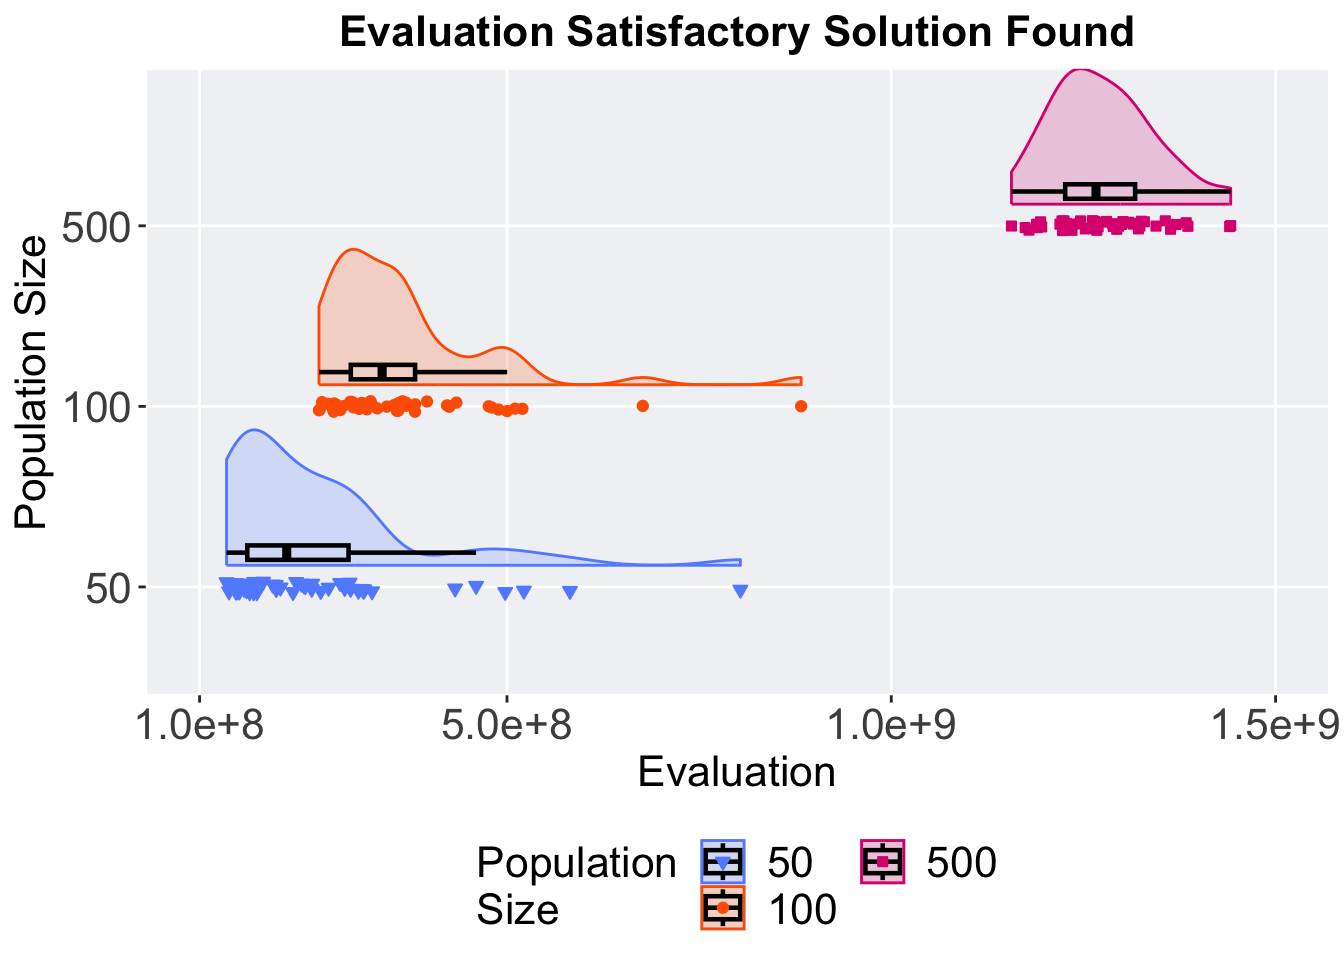
\includegraphics[width=1\linewidth]{lexicase-analysis-supplemental_files/figure-latex/exp-ssf-1}

\hypertarget{summary-statistics-1}{%
\subsection{Summary statistics}\label{summary-statistics-1}}

\begin{Shaded}
\begin{Highlighting}[]
\NormalTok{ssf }\SpecialCharTok{\%\textgreater{}\%}
  \FunctionTok{group\_by}\NormalTok{(pop\_size) }\SpecialCharTok{\%\textgreater{}\%}
\NormalTok{  dplyr}\SpecialCharTok{::}\FunctionTok{summarise}\NormalTok{(}
    \AttributeTok{count =} \FunctionTok{n}\NormalTok{(),}
    \AttributeTok{na\_cnt =} \FunctionTok{sum}\NormalTok{(}\FunctionTok{is.na}\NormalTok{(evaluation)),}
    \AttributeTok{min =} \FunctionTok{min}\NormalTok{(evaluation, }\AttributeTok{na.rm =} \ConstantTok{TRUE}\NormalTok{),}
    \AttributeTok{median =} \FunctionTok{median}\NormalTok{(evaluation, }\AttributeTok{na.rm =} \ConstantTok{TRUE}\NormalTok{),}
    \AttributeTok{mean =} \FunctionTok{mean}\NormalTok{(evaluation, }\AttributeTok{na.rm =} \ConstantTok{TRUE}\NormalTok{),}
    \AttributeTok{max =} \FunctionTok{max}\NormalTok{(evaluation, }\AttributeTok{na.rm =} \ConstantTok{TRUE}\NormalTok{),}
    \AttributeTok{IQR =} \FunctionTok{IQR}\NormalTok{(evaluation, }\AttributeTok{na.rm =} \ConstantTok{TRUE}\NormalTok{)}
\NormalTok{  )}
\end{Highlighting}
\end{Shaded}

\begin{verbatim}
## # A tibble: 3 x 8
##   pop_size count na_cnt        min     median       mean        max       IQR
##   <fct>    <int>  <int>      <dbl>      <dbl>      <dbl>      <dbl>     <dbl>
## 1 50          50      0  135075000  213407500  251829000  803685000 131750000
## 2 100         50      0  255330000  337500000  364654000  882710000  83672500
## 3 500         50      0 1156350000 1266325000 1275005000 1441600000  90962500
\end{verbatim}

\hypertarget{kruskal-wallis-test-1}{%
\subsection{Kruskal-Wallis test}\label{kruskal-wallis-test-1}}

\begin{Shaded}
\begin{Highlighting}[]
\FunctionTok{kruskal.test}\NormalTok{(evaluation }\SpecialCharTok{\textasciitilde{}}\NormalTok{ pop\_size, }\AttributeTok{data =}\NormalTok{ ssf)}
\end{Highlighting}
\end{Shaded}

\begin{verbatim}
## 
##  Kruskal-Wallis rank sum test
## 
## data:  evaluation by pop_size
## Kruskal-Wallis chi-squared = 113.38, df = 2, p-value < 2.2e-16
\end{verbatim}

\hypertarget{pairwise-wilcoxon-test-1}{%
\subsection{Pairwise wilcoxon test}\label{pairwise-wilcoxon-test-1}}

\begin{Shaded}
\begin{Highlighting}[]
\FunctionTok{pairwise.wilcox.test}\NormalTok{(}\AttributeTok{x =}\NormalTok{ ssf}\SpecialCharTok{$}\NormalTok{evaluation, }\AttributeTok{g =}\NormalTok{ ssf}\SpecialCharTok{$}\NormalTok{pop\_size, }\AttributeTok{p.adjust.method =} \StringTok{"bonferroni"}\NormalTok{,}
                     \AttributeTok{paired =} \ConstantTok{FALSE}\NormalTok{, }\AttributeTok{conf.int =} \ConstantTok{FALSE}\NormalTok{, }\AttributeTok{alternative =} \StringTok{\textquotesingle{}g\textquotesingle{}}\NormalTok{)}
\end{Highlighting}
\end{Shaded}

\begin{verbatim}
## 
##  Pairwise comparisons using Wilcoxon rank sum test with continuity correction 
## 
## data:  ssf$evaluation and ssf$pop_size 
## 
##     50      100    
## 100 3.1e-08 -      
## 500 < 2e-16 < 2e-16
## 
## P value adjustment method: bonferroni
\end{verbatim}

\hypertarget{contradictory-objectives-100-results}{%
\chapter{Contradictory objectives 100 results}\label{contradictory-objectives-100-results}}

Here we report the \textbf{activation gene coverage} and \textbf{satisfactory trait coverage} was found on the contradictory objectives diagnostic.
50 replicates were conducted for each population size explored.
Activation gene coverage is calculated by finding all the unique activation genes found within a given population.
Satisfactory trait coverage is calculated by finding all the unique satisfactory traits found within a given population.

\hypertarget{analysis-setup-1}{%
\section{Analysis setup}\label{analysis-setup-1}}

\begin{Shaded}
\begin{Highlighting}[]
\FunctionTok{library}\NormalTok{(ggplot2)}
\FunctionTok{library}\NormalTok{(cowplot)}
\FunctionTok{library}\NormalTok{(dplyr)}
\FunctionTok{library}\NormalTok{(PupillometryR)}

\CommentTok{\# over time data }
\NormalTok{over\_time }\OtherTok{\textless{}{-}} \FunctionTok{read.csv}\NormalTok{(}\StringTok{"../Paper\_Data/Contradictory{-}100/ot.csv"}\NormalTok{, }\AttributeTok{header =} \ConstantTok{TRUE}\NormalTok{, }\AttributeTok{stringsAsFactors =} \ConstantTok{FALSE}\NormalTok{)}
\NormalTok{over\_time}\SpecialCharTok{$}\NormalTok{pop\_size }\OtherTok{\textless{}{-}} \FunctionTok{factor}\NormalTok{(over\_time}\SpecialCharTok{$}\NormalTok{pop\_size, }\AttributeTok{levels =}\NormalTok{ NAMES)}

\CommentTok{\# best performance data}
\NormalTok{best }\OtherTok{\textless{}{-}} \FunctionTok{read.csv}\NormalTok{(}\StringTok{\textquotesingle{}../Paper\_Data/Contradictory{-}100/best.csv\textquotesingle{}}\NormalTok{, }\AttributeTok{header =} \ConstantTok{TRUE}\NormalTok{, }\AttributeTok{stringsAsFactors =} \ConstantTok{FALSE}\NormalTok{)}
\NormalTok{best}\SpecialCharTok{$}\NormalTok{pop\_size }\OtherTok{\textless{}{-}} \FunctionTok{factor}\NormalTok{(best}\SpecialCharTok{$}\NormalTok{pop\_size, }\AttributeTok{levels =}\NormalTok{ NAMES)}
\end{Highlighting}
\end{Shaded}

\hypertarget{activation-gene-coverage}{%
\section{Activation gene coverage}\label{activation-gene-coverage}}

\hypertarget{coverage-over-time}{%
\subsection{Coverage over time}\label{coverage-over-time}}

Performance of the best solution in the population at each generation over time.

\begin{Shaded}
\begin{Highlighting}[]
\CommentTok{\# aggregate }
\NormalTok{lines }\OtherTok{=} \FunctionTok{filter}\NormalTok{(over\_time,eval }\SpecialCharTok{!=} \DecValTok{0}\NormalTok{) }\SpecialCharTok{\%\textgreater{}\%}
  \FunctionTok{group\_by}\NormalTok{(pop\_size, eval) }\SpecialCharTok{\%\textgreater{}\%}
\NormalTok{  dplyr}\SpecialCharTok{::}\FunctionTok{summarise}\NormalTok{(}
    \AttributeTok{min =} \FunctionTok{min}\NormalTok{(activation\_coverage),}
    \AttributeTok{mean =} \FunctionTok{mean}\NormalTok{(activation\_coverage),}
    \AttributeTok{max =} \FunctionTok{max}\NormalTok{(activation\_coverage)}
\NormalTok{  )}
\NormalTok{lines}\SpecialCharTok{$}\NormalTok{pop\_size }\OtherTok{\textless{}{-}} \FunctionTok{factor}\NormalTok{(lines}\SpecialCharTok{$}\NormalTok{pop\_size, }\AttributeTok{levels =}\NormalTok{ NAMES)}

\FunctionTok{ggplot}\NormalTok{(lines, }\FunctionTok{aes}\NormalTok{(}\AttributeTok{x=}\NormalTok{eval, }\AttributeTok{y=}\NormalTok{mean, }\AttributeTok{group =}\NormalTok{ pop\_size, }\AttributeTok{fill =}\NormalTok{ pop\_size, }\AttributeTok{color =}\NormalTok{ pop\_size, }\AttributeTok{shape =}\NormalTok{ pop\_size)) }\SpecialCharTok{+}
  \FunctionTok{geom\_ribbon}\NormalTok{(}\FunctionTok{aes}\NormalTok{(}\AttributeTok{ymin =}\NormalTok{ min, }\AttributeTok{ymax =}\NormalTok{ max), }\AttributeTok{alpha =} \FloatTok{0.1}\NormalTok{) }\SpecialCharTok{+}
  \FunctionTok{geom\_line}\NormalTok{(}\AttributeTok{linewidth =} \FloatTok{0.5}\NormalTok{) }\SpecialCharTok{+}
  \FunctionTok{geom\_point}\NormalTok{(}\AttributeTok{data =} \FunctionTok{filter}\NormalTok{(lines, eval }\SpecialCharTok{\%\%} \DecValTok{100000000} \SpecialCharTok{==} \DecValTok{0} \SpecialCharTok{\&}\NormalTok{ eval }\SpecialCharTok{!=} \DecValTok{0}\NormalTok{), }\AttributeTok{size =} \FloatTok{1.0}\NormalTok{, }\AttributeTok{stroke =} \FloatTok{2.0}\NormalTok{, }\AttributeTok{alpha =} \FloatTok{1.0}\NormalTok{) }\SpecialCharTok{+}
  \FunctionTok{scale\_y\_continuous}\NormalTok{(}
    \AttributeTok{name=}\StringTok{"Coverage"}\NormalTok{,}
    \AttributeTok{limits=}\FunctionTok{c}\NormalTok{(}\DecValTok{0}\NormalTok{, }\DecValTok{100}\NormalTok{),}
    \AttributeTok{breaks=}\FunctionTok{seq}\NormalTok{(}\DecValTok{0}\NormalTok{,}\DecValTok{100}\NormalTok{, }\DecValTok{25}\NormalTok{),}
    \AttributeTok{labels=}\FunctionTok{c}\NormalTok{(}\StringTok{"0"}\NormalTok{, }\StringTok{"25"}\NormalTok{, }\StringTok{"50"}\NormalTok{, }\StringTok{"75"}\NormalTok{, }\StringTok{"100"}\NormalTok{)}
\NormalTok{  ) }\SpecialCharTok{+}
  \FunctionTok{scale\_x\_continuous}\NormalTok{(}
    \AttributeTok{name=}\StringTok{"Evaluation"}\NormalTok{,}
    \AttributeTok{labels =} \FunctionTok{c}\NormalTok{(}\StringTok{\textquotesingle{}0.0e+0\textquotesingle{}}\NormalTok{, }\StringTok{\textquotesingle{}5.0e+8\textquotesingle{}}\NormalTok{,}\StringTok{\textquotesingle{}1.0e+9\textquotesingle{}}\NormalTok{,}\StringTok{\textquotesingle{}1.5e+9\textquotesingle{}}\NormalTok{),}
    \AttributeTok{limits =} \FunctionTok{c}\NormalTok{(}\DecValTok{0}\NormalTok{,}\DecValTok{1520000000}\NormalTok{)}
    
\NormalTok{  ) }\SpecialCharTok{+}
  \FunctionTok{scale\_shape\_manual}\NormalTok{(}\AttributeTok{values=}\NormalTok{SHAPE)}\SpecialCharTok{+}
  \FunctionTok{scale\_colour\_manual}\NormalTok{(}\AttributeTok{values =}\NormalTok{ cb\_palette) }\SpecialCharTok{+}
  \FunctionTok{scale\_fill\_manual}\NormalTok{(}\AttributeTok{values =}\NormalTok{ cb\_palette) }\SpecialCharTok{+}
  \FunctionTok{ggtitle}\NormalTok{(}\StringTok{\textquotesingle{}Activation gene coverage over time\textquotesingle{}}\NormalTok{)}\SpecialCharTok{+}
\NormalTok{  p\_theme }\SpecialCharTok{+}
  \FunctionTok{guides}\NormalTok{(}
    \AttributeTok{shape=}\FunctionTok{guide\_legend}\NormalTok{(}\AttributeTok{nrow=}\DecValTok{2}\NormalTok{, }\AttributeTok{title.position =} \StringTok{"left"}\NormalTok{, }\AttributeTok{title =} \StringTok{\textquotesingle{}Population}\SpecialCharTok{\textbackslash{}n}\StringTok{Size\textquotesingle{}}\NormalTok{),}
    \AttributeTok{color=}\FunctionTok{guide\_legend}\NormalTok{(}\AttributeTok{nrow=}\DecValTok{2}\NormalTok{, }\AttributeTok{title.position =} \StringTok{"left"}\NormalTok{, }\AttributeTok{title =} \StringTok{\textquotesingle{}Population}\SpecialCharTok{\textbackslash{}n}\StringTok{Size\textquotesingle{}}\NormalTok{),}
    \AttributeTok{fill=}\FunctionTok{guide\_legend}\NormalTok{(}\AttributeTok{nrow=}\DecValTok{2}\NormalTok{, }\AttributeTok{title.position =} \StringTok{"left"}\NormalTok{, }\AttributeTok{title =} \StringTok{\textquotesingle{}Population}\SpecialCharTok{\textbackslash{}n}\StringTok{Size\textquotesingle{}}\NormalTok{)}
\NormalTok{  )}
\end{Highlighting}
\end{Shaded}

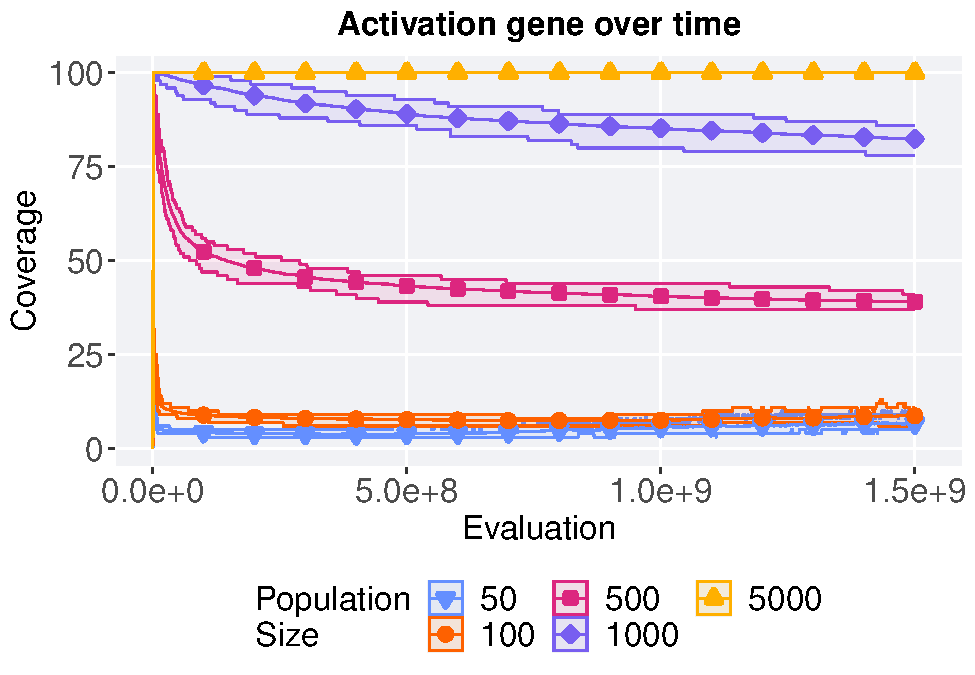
\includegraphics[width=1\linewidth]{lexicase-analysis-supplemental_files/figure-latex/con-150-act-ot-1}

\hypertarget{satisfactory-trait-coverage}{%
\section{Satisfactory trait coverage}\label{satisfactory-trait-coverage}}

\hypertarget{coverage-over-time-1}{%
\subsection{Coverage over time}\label{coverage-over-time-1}}

Satisfactory trait coverage over time.

\begin{Shaded}
\begin{Highlighting}[]
\CommentTok{\# aggregate }
\NormalTok{lines }\OtherTok{=}\NormalTok{ over\_time }\SpecialCharTok{\%\textgreater{}\%}
  \FunctionTok{group\_by}\NormalTok{(pop\_size, eval) }\SpecialCharTok{\%\textgreater{}\%}
\NormalTok{  dplyr}\SpecialCharTok{::}\FunctionTok{summarise}\NormalTok{(}
    \AttributeTok{min =} \FunctionTok{min}\NormalTok{(satisfactory\_coverage),}
    \AttributeTok{mean =} \FunctionTok{mean}\NormalTok{(satisfactory\_coverage),}
    \AttributeTok{max =} \FunctionTok{max}\NormalTok{(satisfactory\_coverage)}
\NormalTok{  )}
\NormalTok{lines}\SpecialCharTok{$}\NormalTok{pop\_size }\OtherTok{\textless{}{-}} \FunctionTok{factor}\NormalTok{(lines}\SpecialCharTok{$}\NormalTok{pop\_size, }\AttributeTok{levels =}\NormalTok{ NAMES)}

\FunctionTok{ggplot}\NormalTok{(lines, }\FunctionTok{aes}\NormalTok{(}\AttributeTok{x=}\NormalTok{eval, }\AttributeTok{y=}\NormalTok{mean, }\AttributeTok{group =}\NormalTok{ pop\_size, }\AttributeTok{fill =}\NormalTok{ pop\_size, }\AttributeTok{color =}\NormalTok{ pop\_size, }\AttributeTok{shape =}\NormalTok{ pop\_size)) }\SpecialCharTok{+}
  \FunctionTok{geom\_ribbon}\NormalTok{(}\FunctionTok{aes}\NormalTok{(}\AttributeTok{ymin =}\NormalTok{ min, }\AttributeTok{ymax =}\NormalTok{ max), }\AttributeTok{alpha =} \FloatTok{0.1}\NormalTok{) }\SpecialCharTok{+}
  \FunctionTok{geom\_line}\NormalTok{(}\AttributeTok{linewidth =} \FloatTok{0.5}\NormalTok{) }\SpecialCharTok{+}
  \FunctionTok{geom\_point}\NormalTok{(}\AttributeTok{data =} \FunctionTok{filter}\NormalTok{(lines, eval }\SpecialCharTok{\%\%} \DecValTok{100000000} \SpecialCharTok{==} \DecValTok{0} \SpecialCharTok{\&}\NormalTok{ eval }\SpecialCharTok{!=} \DecValTok{0}\NormalTok{), }\AttributeTok{size =} \FloatTok{1.0}\NormalTok{, }\AttributeTok{stroke =} \FloatTok{2.0}\NormalTok{, }\AttributeTok{alpha =} \FloatTok{1.0}\NormalTok{) }\SpecialCharTok{+}
  \FunctionTok{scale\_y\_continuous}\NormalTok{(}
    \AttributeTok{name=}\StringTok{"Coverage"}\NormalTok{,}
    \AttributeTok{limits=}\FunctionTok{c}\NormalTok{(}\DecValTok{0}\NormalTok{, }\DecValTok{100}\NormalTok{),}
    \AttributeTok{breaks=}\FunctionTok{seq}\NormalTok{(}\DecValTok{0}\NormalTok{,}\DecValTok{100}\NormalTok{, }\DecValTok{25}\NormalTok{),}
    \AttributeTok{labels=}\FunctionTok{c}\NormalTok{(}\StringTok{"0"}\NormalTok{, }\StringTok{"25"}\NormalTok{, }\StringTok{"50"}\NormalTok{, }\StringTok{"75"}\NormalTok{, }\StringTok{"100"}\NormalTok{)}
\NormalTok{  ) }\SpecialCharTok{+}
  \FunctionTok{scale\_x\_continuous}\NormalTok{(}
    \AttributeTok{name=}\StringTok{"Evaluation"}\NormalTok{,}
    \AttributeTok{labels =} \FunctionTok{c}\NormalTok{(}\StringTok{\textquotesingle{}0.0e+0\textquotesingle{}}\NormalTok{, }\StringTok{\textquotesingle{}5.0e+8\textquotesingle{}}\NormalTok{,}\StringTok{\textquotesingle{}1.0e+9\textquotesingle{}}\NormalTok{,}\StringTok{\textquotesingle{}1.5e+9\textquotesingle{}}\NormalTok{),}
    \AttributeTok{limits =} \FunctionTok{c}\NormalTok{(}\DecValTok{0}\NormalTok{,}\DecValTok{1520000000}\NormalTok{)}
    
\NormalTok{  ) }\SpecialCharTok{+}
  \FunctionTok{scale\_shape\_manual}\NormalTok{(}\AttributeTok{values=}\NormalTok{SHAPE)}\SpecialCharTok{+}
  \FunctionTok{scale\_colour\_manual}\NormalTok{(}\AttributeTok{values =}\NormalTok{ cb\_palette) }\SpecialCharTok{+}
  \FunctionTok{scale\_fill\_manual}\NormalTok{(}\AttributeTok{values =}\NormalTok{ cb\_palette) }\SpecialCharTok{+}
  \FunctionTok{ggtitle}\NormalTok{(}\StringTok{\textquotesingle{}Satisfactory trait coverage over time\textquotesingle{}}\NormalTok{)}\SpecialCharTok{+}
\NormalTok{  p\_theme }\SpecialCharTok{+}
  \FunctionTok{guides}\NormalTok{(}
    \AttributeTok{shape=}\FunctionTok{guide\_legend}\NormalTok{(}\AttributeTok{nrow=}\DecValTok{2}\NormalTok{, }\AttributeTok{title.position =} \StringTok{"left"}\NormalTok{, }\AttributeTok{title =} \StringTok{\textquotesingle{}Population}\SpecialCharTok{\textbackslash{}n}\StringTok{Size\textquotesingle{}}\NormalTok{),}
    \AttributeTok{color=}\FunctionTok{guide\_legend}\NormalTok{(}\AttributeTok{nrow=}\DecValTok{2}\NormalTok{, }\AttributeTok{title.position =} \StringTok{"left"}\NormalTok{, }\AttributeTok{title =} \StringTok{\textquotesingle{}Population}\SpecialCharTok{\textbackslash{}n}\StringTok{Size\textquotesingle{}}\NormalTok{),}
    \AttributeTok{fill=}\FunctionTok{guide\_legend}\NormalTok{(}\AttributeTok{nrow=}\DecValTok{2}\NormalTok{, }\AttributeTok{title.position =} \StringTok{"left"}\NormalTok{, }\AttributeTok{title =} \StringTok{\textquotesingle{}Population}\SpecialCharTok{\textbackslash{}n}\StringTok{Size\textquotesingle{}}\NormalTok{)}
\NormalTok{  )}
\end{Highlighting}
\end{Shaded}

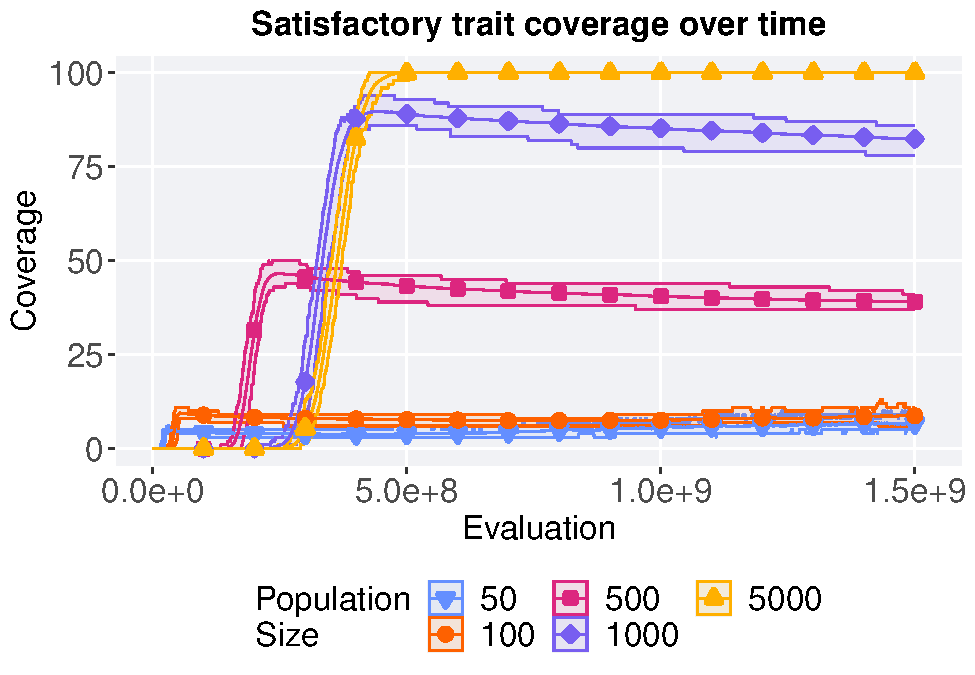
\includegraphics[width=1\linewidth]{lexicase-analysis-supplemental_files/figure-latex/con-150-sat-ot-1}

\hypertarget{best-satisfactory-trait-coverage-found-throughout-run}{%
\subsection{Best satisfactory trait coverage found throughout run}\label{best-satisfactory-trait-coverage-found-throughout-run}}

Satisfactory trait coverage of the best population found throughout an evolutionary run.

\begin{Shaded}
\begin{Highlighting}[]
\FunctionTok{ggplot}\NormalTok{(best, }\FunctionTok{aes}\NormalTok{(}\AttributeTok{x =}\NormalTok{ pop\_size, }\AttributeTok{y =}\NormalTok{ coverage, }\AttributeTok{color =}\NormalTok{ pop\_size, }\AttributeTok{fill =}\NormalTok{ pop\_size, }\AttributeTok{shape =}\NormalTok{ pop\_size)) }\SpecialCharTok{+}
  \FunctionTok{geom\_flat\_violin}\NormalTok{(}\AttributeTok{position =} \FunctionTok{position\_nudge}\NormalTok{(}\AttributeTok{x =}\NormalTok{ .}\DecValTok{1}\NormalTok{, }\AttributeTok{y =} \DecValTok{0}\NormalTok{), }\AttributeTok{scale =} \StringTok{\textquotesingle{}width\textquotesingle{}}\NormalTok{, }\AttributeTok{alpha =} \FloatTok{0.2}\NormalTok{, }\AttributeTok{width =} \FloatTok{1.5}\NormalTok{) }\SpecialCharTok{+}
  \FunctionTok{geom\_boxplot}\NormalTok{(}\AttributeTok{color =} \StringTok{\textquotesingle{}black\textquotesingle{}}\NormalTok{, }\AttributeTok{width =}\NormalTok{ .}\DecValTok{07}\NormalTok{, }\AttributeTok{outlier.shape =} \ConstantTok{NA}\NormalTok{, }\AttributeTok{alpha =} \FloatTok{0.0}\NormalTok{, }\AttributeTok{size =} \FloatTok{1.0}\NormalTok{, }\AttributeTok{position =} \FunctionTok{position\_nudge}\NormalTok{(}\AttributeTok{x =}\NormalTok{ .}\DecValTok{16}\NormalTok{, }\AttributeTok{y =} \DecValTok{0}\NormalTok{)) }\SpecialCharTok{+}
  \FunctionTok{geom\_point}\NormalTok{(}\AttributeTok{position =} \FunctionTok{position\_jitter}\NormalTok{(}\AttributeTok{width =} \FloatTok{0.02}\NormalTok{, }\AttributeTok{height =} \FloatTok{0.0001}\NormalTok{), }\AttributeTok{size =} \FloatTok{1.5}\NormalTok{, }\AttributeTok{alpha =} \FloatTok{1.0}\NormalTok{) }\SpecialCharTok{+}
  \FunctionTok{scale\_y\_continuous}\NormalTok{(}
    \AttributeTok{name=}\StringTok{"Coverage"}\NormalTok{,}
    \AttributeTok{limits=}\FunctionTok{c}\NormalTok{(}\DecValTok{0}\NormalTok{, }\DecValTok{100}\NormalTok{),}
    \AttributeTok{breaks=}\FunctionTok{seq}\NormalTok{(}\DecValTok{0}\NormalTok{,}\DecValTok{100}\NormalTok{, }\DecValTok{25}\NormalTok{),}
    \AttributeTok{labels=}\FunctionTok{c}\NormalTok{(}\StringTok{"0"}\NormalTok{, }\StringTok{"25"}\NormalTok{, }\StringTok{"50"}\NormalTok{, }\StringTok{"75"}\NormalTok{, }\StringTok{"100"}\NormalTok{),}
\NormalTok{  ) }\SpecialCharTok{+}
  \FunctionTok{scale\_x\_discrete}\NormalTok{(}
    \AttributeTok{name=}\StringTok{"Population Size"}
\NormalTok{  )}\SpecialCharTok{+}
  \FunctionTok{scale\_shape\_manual}\NormalTok{(}\AttributeTok{values=}\NormalTok{SHAPE)}\SpecialCharTok{+}
  \FunctionTok{scale\_colour\_manual}\NormalTok{(}\AttributeTok{values =}\NormalTok{ cb\_palette, ) }\SpecialCharTok{+}
  \FunctionTok{scale\_fill\_manual}\NormalTok{(}\AttributeTok{values =}\NormalTok{ cb\_palette) }\SpecialCharTok{+}
  \FunctionTok{ggtitle}\NormalTok{(}\StringTok{\textquotesingle{}Best satisfactory coverage\textquotesingle{}}\NormalTok{)}\SpecialCharTok{+}
\NormalTok{  p\_theme }\SpecialCharTok{+} \FunctionTok{coord\_flip}\NormalTok{() }\SpecialCharTok{+}
  \FunctionTok{guides}\NormalTok{(}
    \AttributeTok{shape=}\FunctionTok{guide\_legend}\NormalTok{(}\AttributeTok{nrow=}\DecValTok{2}\NormalTok{, }\AttributeTok{title.position =} \StringTok{"left"}\NormalTok{, }\AttributeTok{title =} \StringTok{\textquotesingle{}Population}\SpecialCharTok{\textbackslash{}n}\StringTok{Size\textquotesingle{}}\NormalTok{),}
    \AttributeTok{color=}\FunctionTok{guide\_legend}\NormalTok{(}\AttributeTok{nrow=}\DecValTok{2}\NormalTok{, }\AttributeTok{title.position =} \StringTok{"left"}\NormalTok{, }\AttributeTok{title =} \StringTok{\textquotesingle{}Population}\SpecialCharTok{\textbackslash{}n}\StringTok{Size\textquotesingle{}}\NormalTok{),}
    \AttributeTok{fill=}\FunctionTok{guide\_legend}\NormalTok{(}\AttributeTok{nrow=}\DecValTok{2}\NormalTok{, }\AttributeTok{title.position =} \StringTok{"left"}\NormalTok{, }\AttributeTok{title =} \StringTok{\textquotesingle{}Population}\SpecialCharTok{\textbackslash{}n}\StringTok{Size\textquotesingle{}}\NormalTok{)}
\NormalTok{  )}
\end{Highlighting}
\end{Shaded}

\begin{verbatim}
## Warning: Removed 18 rows containing missing values (`geom_point()`).
\end{verbatim}

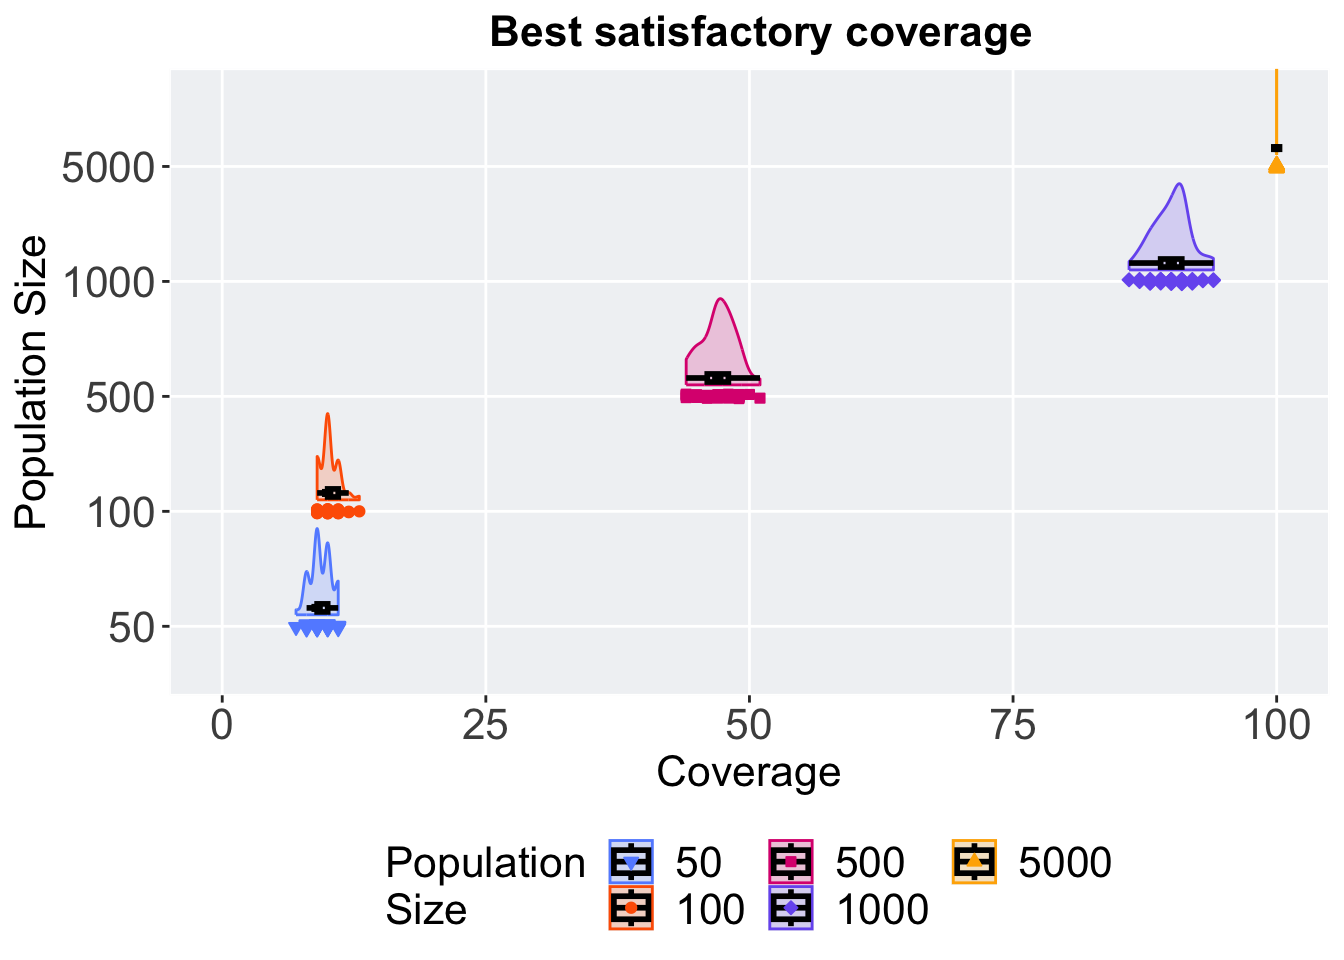
\includegraphics[width=1\linewidth]{lexicase-analysis-supplemental_files/figure-latex/con-150-sat-best-1}

\hypertarget{summary-statistics-2}{%
\subsubsection{Summary statistics}\label{summary-statistics-2}}

\begin{Shaded}
\begin{Highlighting}[]
\NormalTok{best }\SpecialCharTok{\%\textgreater{}\%}
  \FunctionTok{group\_by}\NormalTok{(pop\_size) }\SpecialCharTok{\%\textgreater{}\%}
\NormalTok{  dplyr}\SpecialCharTok{::}\FunctionTok{summarise}\NormalTok{(}
    \AttributeTok{count =} \FunctionTok{n}\NormalTok{(),}
    \AttributeTok{na\_cnt =} \FunctionTok{sum}\NormalTok{(}\FunctionTok{is.na}\NormalTok{(coverage)),}
    \AttributeTok{min =} \FunctionTok{min}\NormalTok{(coverage, }\AttributeTok{na.rm =} \ConstantTok{TRUE}\NormalTok{),}
    \AttributeTok{median =} \FunctionTok{median}\NormalTok{(coverage, }\AttributeTok{na.rm =} \ConstantTok{TRUE}\NormalTok{),}
    \AttributeTok{mean =} \FunctionTok{mean}\NormalTok{(coverage, }\AttributeTok{na.rm =} \ConstantTok{TRUE}\NormalTok{),}
    \AttributeTok{max =} \FunctionTok{max}\NormalTok{(coverage, }\AttributeTok{na.rm =} \ConstantTok{TRUE}\NormalTok{),}
    \AttributeTok{IQR =} \FunctionTok{IQR}\NormalTok{(coverage, }\AttributeTok{na.rm =} \ConstantTok{TRUE}\NormalTok{)}
\NormalTok{  )}
\end{Highlighting}
\end{Shaded}

\begin{verbatim}
## # A tibble: 5 x 8
##   pop_size count na_cnt   min median   mean   max   IQR
##   <fct>    <int>  <int> <int>  <dbl>  <dbl> <int> <dbl>
## 1 50          50      0     7      9   9.36    11     1
## 2 100         50      0     9     10  10.1     13     1
## 3 500         50      0    44     47  47.0     51     2
## 4 1000        50      0    86     90  90.0     94     2
## 5 5000        50      0   100    100 100      100     0
\end{verbatim}

\hypertarget{kruskal-wallis-test-2}{%
\subsubsection{Kruskal-Wallis test}\label{kruskal-wallis-test-2}}

\begin{Shaded}
\begin{Highlighting}[]
\FunctionTok{kruskal.test}\NormalTok{(coverage }\SpecialCharTok{\textasciitilde{}}\NormalTok{ pop\_size, }\AttributeTok{data =}\NormalTok{ best)}
\end{Highlighting}
\end{Shaded}

\begin{verbatim}
## 
##  Kruskal-Wallis rank sum test
## 
## data:  coverage by pop_size
## Kruskal-Wallis chi-squared = 232.33, df = 4, p-value < 2.2e-16
\end{verbatim}

\hypertarget{pairwise-wilcoxon-test-2}{%
\subsubsection{Pairwise wilcoxon test}\label{pairwise-wilcoxon-test-2}}

\begin{Shaded}
\begin{Highlighting}[]
\FunctionTok{pairwise.wilcox.test}\NormalTok{(}\AttributeTok{x =}\NormalTok{ best}\SpecialCharTok{$}\NormalTok{coverage, }\AttributeTok{g =}\NormalTok{ best}\SpecialCharTok{$}\NormalTok{pop\_size, }\AttributeTok{p.adjust.method =} \StringTok{"bonferroni"}\NormalTok{,}
                     \AttributeTok{paired =} \ConstantTok{FALSE}\NormalTok{, }\AttributeTok{conf.int =} \ConstantTok{FALSE}\NormalTok{, }\AttributeTok{alternative =} \StringTok{\textquotesingle{}g\textquotesingle{}}\NormalTok{)}
\end{Highlighting}
\end{Shaded}

\begin{verbatim}
## 
##  Pairwise comparisons using Wilcoxon rank sum test with continuity correction 
## 
## data:  best$coverage and best$pop_size 
## 
##      50     100    500    1000  
## 100  0.0019 -      -      -     
## 500  <2e-16 <2e-16 -      -     
## 1000 <2e-16 <2e-16 <2e-16 -     
## 5000 <2e-16 <2e-16 <2e-16 <2e-16
## 
## P value adjustment method: bonferroni
\end{verbatim}

\hypertarget{contradictory-objectives-200-results}{%
\chapter{Contradictory objectives 200 results}\label{contradictory-objectives-200-results}}

Here we report the \textbf{activation gene coverage} and \textbf{satisfactory trait coverage} was found on the contradictory objectives diagnostic.
50 replicates were conducted for each population size explored.
Activation gene coverage is calculated by finding all the unique activation genes found within a given population.
Satisfactory trait coverage is calculated by finding all the unique satisfactory traits found within a given population.

\hypertarget{analysis-setup-2}{%
\section{Analysis setup}\label{analysis-setup-2}}

\begin{Shaded}
\begin{Highlighting}[]
\FunctionTok{library}\NormalTok{(ggplot2)}
\FunctionTok{library}\NormalTok{(cowplot)}
\FunctionTok{library}\NormalTok{(dplyr)}
\FunctionTok{library}\NormalTok{(PupillometryR)}

\CommentTok{\# over time data}
\NormalTok{over\_time }\OtherTok{\textless{}{-}} \FunctionTok{read.csv}\NormalTok{(}\StringTok{"../Paper\_Data/Contradictory{-}200/ot.csv"}\NormalTok{, }\AttributeTok{header =} \ConstantTok{TRUE}\NormalTok{, }\AttributeTok{stringsAsFactors =} \ConstantTok{FALSE}\NormalTok{)}
\NormalTok{over\_time}\SpecialCharTok{$}\NormalTok{pop\_size }\OtherTok{\textless{}{-}} \FunctionTok{factor}\NormalTok{(over\_time}\SpecialCharTok{$}\NormalTok{pop\_size, }\AttributeTok{levels =}\NormalTok{ NAMES)}

\CommentTok{\# best performance data}
\NormalTok{best }\OtherTok{\textless{}{-}} \FunctionTok{read.csv}\NormalTok{(}\StringTok{\textquotesingle{}../Paper\_Data/Contradictory{-}200/best.csv\textquotesingle{}}\NormalTok{, }\AttributeTok{header =} \ConstantTok{TRUE}\NormalTok{, }\AttributeTok{stringsAsFactors =} \ConstantTok{FALSE}\NormalTok{)}
\NormalTok{best}\SpecialCharTok{$}\NormalTok{pop\_size }\OtherTok{\textless{}{-}} \FunctionTok{factor}\NormalTok{(best}\SpecialCharTok{$}\NormalTok{pop\_size, }\AttributeTok{levels =}\NormalTok{ NAMES)}
\end{Highlighting}
\end{Shaded}

\hypertarget{activation-gene-coverage-1}{%
\section{Activation gene coverage}\label{activation-gene-coverage-1}}

\hypertarget{coverage-over-time-2}{%
\subsection{Coverage over time}\label{coverage-over-time-2}}

Performance of the best solution in the population at each generation over time.

\begin{Shaded}
\begin{Highlighting}[]
\CommentTok{\# aggregate}
\NormalTok{lines }\OtherTok{=} \FunctionTok{filter}\NormalTok{(over\_time,eval }\SpecialCharTok{!=} \DecValTok{0}\NormalTok{) }\SpecialCharTok{\%\textgreater{}\%}
  \FunctionTok{group\_by}\NormalTok{(pop\_size, eval) }\SpecialCharTok{\%\textgreater{}\%}
\NormalTok{  dplyr}\SpecialCharTok{::}\FunctionTok{summarise}\NormalTok{(}
    \AttributeTok{min =} \FunctionTok{min}\NormalTok{(activation\_coverage),}
    \AttributeTok{mean =} \FunctionTok{mean}\NormalTok{(activation\_coverage),}
    \AttributeTok{max =} \FunctionTok{max}\NormalTok{(activation\_coverage)}
\NormalTok{  )}
\NormalTok{lines}\SpecialCharTok{$}\NormalTok{pop\_size }\OtherTok{\textless{}{-}} \FunctionTok{factor}\NormalTok{(lines}\SpecialCharTok{$}\NormalTok{pop\_size, }\AttributeTok{levels =}\NormalTok{ NAMES)}

\FunctionTok{ggplot}\NormalTok{(lines, }\FunctionTok{aes}\NormalTok{(}\AttributeTok{x=}\NormalTok{eval, }\AttributeTok{y=}\NormalTok{mean, }\AttributeTok{group =}\NormalTok{ pop\_size, }\AttributeTok{fill =}\NormalTok{ pop\_size, }\AttributeTok{color =}\NormalTok{ pop\_size, }\AttributeTok{shape =}\NormalTok{ pop\_size)) }\SpecialCharTok{+}
  \FunctionTok{geom\_ribbon}\NormalTok{(}\FunctionTok{aes}\NormalTok{(}\AttributeTok{ymin =}\NormalTok{ min, }\AttributeTok{ymax =}\NormalTok{ max), }\AttributeTok{alpha =} \FloatTok{0.1}\NormalTok{) }\SpecialCharTok{+}
  \FunctionTok{geom\_line}\NormalTok{(}\AttributeTok{linewidth =} \FloatTok{0.5}\NormalTok{) }\SpecialCharTok{+}
  \FunctionTok{geom\_point}\NormalTok{(}\AttributeTok{data =} \FunctionTok{filter}\NormalTok{(lines, eval }\SpecialCharTok{\%\%} \DecValTok{100000000} \SpecialCharTok{==} \DecValTok{0} \SpecialCharTok{\&}\NormalTok{ eval }\SpecialCharTok{!=} \DecValTok{0}\NormalTok{), }\AttributeTok{size =} \FloatTok{1.0}\NormalTok{, }\AttributeTok{stroke =} \FloatTok{2.0}\NormalTok{, }\AttributeTok{alpha =} \FloatTok{1.0}\NormalTok{) }\SpecialCharTok{+}
  \FunctionTok{scale\_y\_continuous}\NormalTok{(}
    \AttributeTok{name=}\StringTok{"Coverage"}\NormalTok{,}
    \AttributeTok{limits=}\FunctionTok{c}\NormalTok{(}\DecValTok{0}\NormalTok{, }\DecValTok{100}\NormalTok{),}
    \AttributeTok{breaks=}\FunctionTok{seq}\NormalTok{(}\DecValTok{0}\NormalTok{,}\DecValTok{100}\NormalTok{, }\DecValTok{25}\NormalTok{),}
    \AttributeTok{labels=}\FunctionTok{c}\NormalTok{(}\StringTok{"0"}\NormalTok{, }\StringTok{"25"}\NormalTok{, }\StringTok{"50"}\NormalTok{, }\StringTok{"75"}\NormalTok{, }\StringTok{"100"}\NormalTok{)}
\NormalTok{  ) }\SpecialCharTok{+}
  \FunctionTok{scale\_x\_continuous}\NormalTok{(}
    \AttributeTok{name=}\StringTok{"Evaluation"}\NormalTok{,}
    \AttributeTok{labels =} \FunctionTok{c}\NormalTok{(}\StringTok{\textquotesingle{}0.0e+0\textquotesingle{}}\NormalTok{, }\StringTok{\textquotesingle{}5.0e+8\textquotesingle{}}\NormalTok{,}\StringTok{\textquotesingle{}1.0e+9\textquotesingle{}}\NormalTok{,}\StringTok{\textquotesingle{}1.5e+9\textquotesingle{}}\NormalTok{),}
    \AttributeTok{limits =} \FunctionTok{c}\NormalTok{(}\DecValTok{0}\NormalTok{,}\DecValTok{1520000000}\NormalTok{)}

\NormalTok{  ) }\SpecialCharTok{+}
  \FunctionTok{scale\_shape\_manual}\NormalTok{(}\AttributeTok{values=}\NormalTok{SHAPE)}\SpecialCharTok{+}
  \FunctionTok{scale\_colour\_manual}\NormalTok{(}\AttributeTok{values =}\NormalTok{ cb\_palette) }\SpecialCharTok{+}
  \FunctionTok{scale\_fill\_manual}\NormalTok{(}\AttributeTok{values =}\NormalTok{ cb\_palette) }\SpecialCharTok{+}
  \FunctionTok{ggtitle}\NormalTok{(}\StringTok{\textquotesingle{}Activation gene coverage over time\textquotesingle{}}\NormalTok{)}\SpecialCharTok{+}
\NormalTok{  p\_theme }\SpecialCharTok{+}
  \FunctionTok{guides}\NormalTok{(}
    \AttributeTok{shape=}\FunctionTok{guide\_legend}\NormalTok{(}\AttributeTok{nrow=}\DecValTok{2}\NormalTok{, }\AttributeTok{title.position =} \StringTok{"left"}\NormalTok{, }\AttributeTok{title =} \StringTok{\textquotesingle{}Population}\SpecialCharTok{\textbackslash{}n}\StringTok{Size\textquotesingle{}}\NormalTok{),}
    \AttributeTok{color=}\FunctionTok{guide\_legend}\NormalTok{(}\AttributeTok{nrow=}\DecValTok{2}\NormalTok{, }\AttributeTok{title.position =} \StringTok{"left"}\NormalTok{, }\AttributeTok{title =} \StringTok{\textquotesingle{}Population}\SpecialCharTok{\textbackslash{}n}\StringTok{Size\textquotesingle{}}\NormalTok{),}
    \AttributeTok{fill=}\FunctionTok{guide\_legend}\NormalTok{(}\AttributeTok{nrow=}\DecValTok{2}\NormalTok{, }\AttributeTok{title.position =} \StringTok{"left"}\NormalTok{, }\AttributeTok{title =} \StringTok{\textquotesingle{}Population}\SpecialCharTok{\textbackslash{}n}\StringTok{Size\textquotesingle{}}\NormalTok{)}
\NormalTok{  )}
\end{Highlighting}
\end{Shaded}

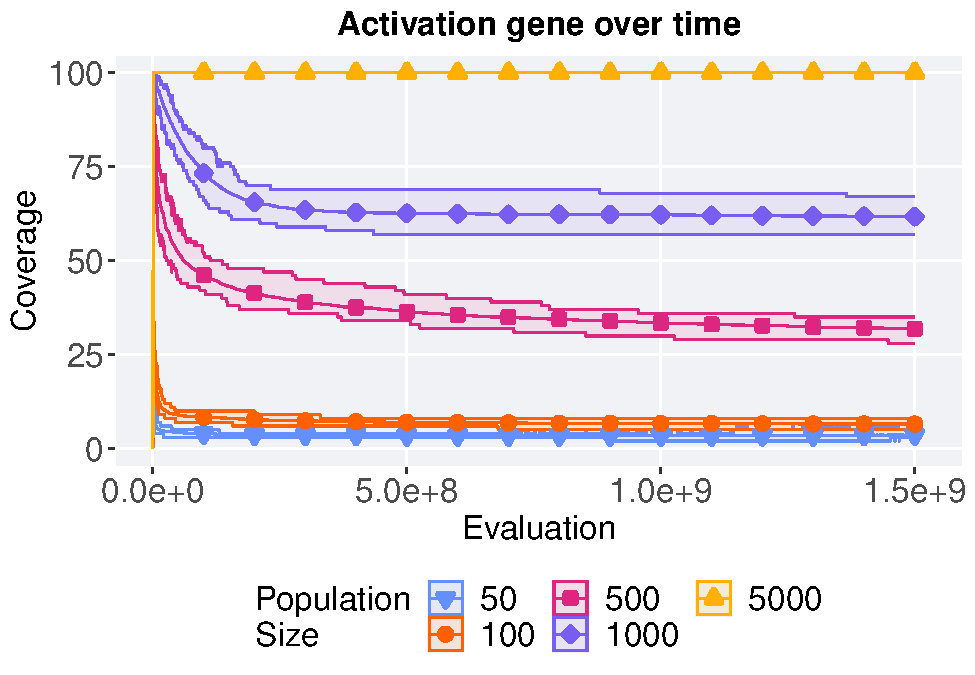
\includegraphics[width=1\linewidth]{lexicase-analysis-supplemental_files/figure-latex/con-200-act-ot-1}

\hypertarget{satisfactory-trait-coverage-1}{%
\section{Satisfactory trait coverage}\label{satisfactory-trait-coverage-1}}

\hypertarget{coverage-over-time-3}{%
\subsection{Coverage over time}\label{coverage-over-time-3}}

Satisfactory trait coverage over time.

\begin{Shaded}
\begin{Highlighting}[]
\CommentTok{\# aggregate}
\NormalTok{lines }\OtherTok{=}\NormalTok{ over\_time }\SpecialCharTok{\%\textgreater{}\%}
  \FunctionTok{group\_by}\NormalTok{(pop\_size, eval) }\SpecialCharTok{\%\textgreater{}\%}
\NormalTok{  dplyr}\SpecialCharTok{::}\FunctionTok{summarise}\NormalTok{(}
    \AttributeTok{min =} \FunctionTok{min}\NormalTok{(satisfactory\_coverage),}
    \AttributeTok{mean =} \FunctionTok{mean}\NormalTok{(satisfactory\_coverage),}
    \AttributeTok{max =} \FunctionTok{max}\NormalTok{(satisfactory\_coverage)}
\NormalTok{  )}
\NormalTok{lines}\SpecialCharTok{$}\NormalTok{pop\_size }\OtherTok{\textless{}{-}} \FunctionTok{factor}\NormalTok{(lines}\SpecialCharTok{$}\NormalTok{pop\_size, }\AttributeTok{levels =}\NormalTok{ NAMES)}

\FunctionTok{ggplot}\NormalTok{(lines, }\FunctionTok{aes}\NormalTok{(}\AttributeTok{x=}\NormalTok{eval, }\AttributeTok{y=}\NormalTok{mean, }\AttributeTok{group =}\NormalTok{ pop\_size, }\AttributeTok{fill =}\NormalTok{ pop\_size, }\AttributeTok{color =}\NormalTok{ pop\_size, }\AttributeTok{shape =}\NormalTok{ pop\_size)) }\SpecialCharTok{+}
  \FunctionTok{geom\_ribbon}\NormalTok{(}\FunctionTok{aes}\NormalTok{(}\AttributeTok{ymin =}\NormalTok{ min, }\AttributeTok{ymax =}\NormalTok{ max), }\AttributeTok{alpha =} \FloatTok{0.1}\NormalTok{) }\SpecialCharTok{+}
  \FunctionTok{geom\_line}\NormalTok{(}\AttributeTok{linewidth =} \FloatTok{0.5}\NormalTok{) }\SpecialCharTok{+}
  \FunctionTok{geom\_point}\NormalTok{(}\AttributeTok{data =} \FunctionTok{filter}\NormalTok{(lines, eval }\SpecialCharTok{\%\%} \DecValTok{100000000} \SpecialCharTok{==} \DecValTok{0} \SpecialCharTok{\&}\NormalTok{ eval }\SpecialCharTok{!=} \DecValTok{0}\NormalTok{), }\AttributeTok{size =} \FloatTok{1.0}\NormalTok{, }\AttributeTok{stroke =} \FloatTok{2.0}\NormalTok{, }\AttributeTok{alpha =} \FloatTok{1.0}\NormalTok{) }\SpecialCharTok{+}
  \FunctionTok{scale\_y\_continuous}\NormalTok{(}
    \AttributeTok{name=}\StringTok{"Coverage"}\NormalTok{,}
    \AttributeTok{limits=}\FunctionTok{c}\NormalTok{(}\DecValTok{0}\NormalTok{, }\DecValTok{100}\NormalTok{),}
    \AttributeTok{breaks=}\FunctionTok{seq}\NormalTok{(}\DecValTok{0}\NormalTok{,}\DecValTok{100}\NormalTok{, }\DecValTok{25}\NormalTok{),}
    \AttributeTok{labels=}\FunctionTok{c}\NormalTok{(}\StringTok{"0"}\NormalTok{, }\StringTok{"25"}\NormalTok{, }\StringTok{"50"}\NormalTok{, }\StringTok{"75"}\NormalTok{, }\StringTok{"100"}\NormalTok{)}
\NormalTok{  ) }\SpecialCharTok{+}
  \FunctionTok{scale\_x\_continuous}\NormalTok{(}
    \AttributeTok{name=}\StringTok{"Evaluation"}\NormalTok{,}
    \AttributeTok{labels =} \FunctionTok{c}\NormalTok{(}\StringTok{\textquotesingle{}0.0e+0\textquotesingle{}}\NormalTok{, }\StringTok{\textquotesingle{}5.0e+8\textquotesingle{}}\NormalTok{,}\StringTok{\textquotesingle{}1.0e+9\textquotesingle{}}\NormalTok{,}\StringTok{\textquotesingle{}1.5e+9\textquotesingle{}}\NormalTok{),}
    \AttributeTok{limits =} \FunctionTok{c}\NormalTok{(}\DecValTok{0}\NormalTok{,}\DecValTok{1520000000}\NormalTok{)}

\NormalTok{  ) }\SpecialCharTok{+}
  \FunctionTok{scale\_shape\_manual}\NormalTok{(}\AttributeTok{values=}\NormalTok{SHAPE)}\SpecialCharTok{+}
  \FunctionTok{scale\_colour\_manual}\NormalTok{(}\AttributeTok{values =}\NormalTok{ cb\_palette) }\SpecialCharTok{+}
  \FunctionTok{scale\_fill\_manual}\NormalTok{(}\AttributeTok{values =}\NormalTok{ cb\_palette) }\SpecialCharTok{+}
  \FunctionTok{ggtitle}\NormalTok{(}\StringTok{\textquotesingle{}Satisfactory trait coverage over time\textquotesingle{}}\NormalTok{)}\SpecialCharTok{+}
\NormalTok{  p\_theme }\SpecialCharTok{+}
  \FunctionTok{guides}\NormalTok{(}
    \AttributeTok{shape=}\FunctionTok{guide\_legend}\NormalTok{(}\AttributeTok{nrow=}\DecValTok{2}\NormalTok{, }\AttributeTok{title.position =} \StringTok{"left"}\NormalTok{, }\AttributeTok{title =} \StringTok{\textquotesingle{}Population}\SpecialCharTok{\textbackslash{}n}\StringTok{Size\textquotesingle{}}\NormalTok{),}
    \AttributeTok{color=}\FunctionTok{guide\_legend}\NormalTok{(}\AttributeTok{nrow=}\DecValTok{2}\NormalTok{, }\AttributeTok{title.position =} \StringTok{"left"}\NormalTok{, }\AttributeTok{title =} \StringTok{\textquotesingle{}Population}\SpecialCharTok{\textbackslash{}n}\StringTok{Size\textquotesingle{}}\NormalTok{),}
    \AttributeTok{fill=}\FunctionTok{guide\_legend}\NormalTok{(}\AttributeTok{nrow=}\DecValTok{2}\NormalTok{, }\AttributeTok{title.position =} \StringTok{"left"}\NormalTok{, }\AttributeTok{title =} \StringTok{\textquotesingle{}Population}\SpecialCharTok{\textbackslash{}n}\StringTok{Size\textquotesingle{}}\NormalTok{)}
\NormalTok{  )}
\end{Highlighting}
\end{Shaded}

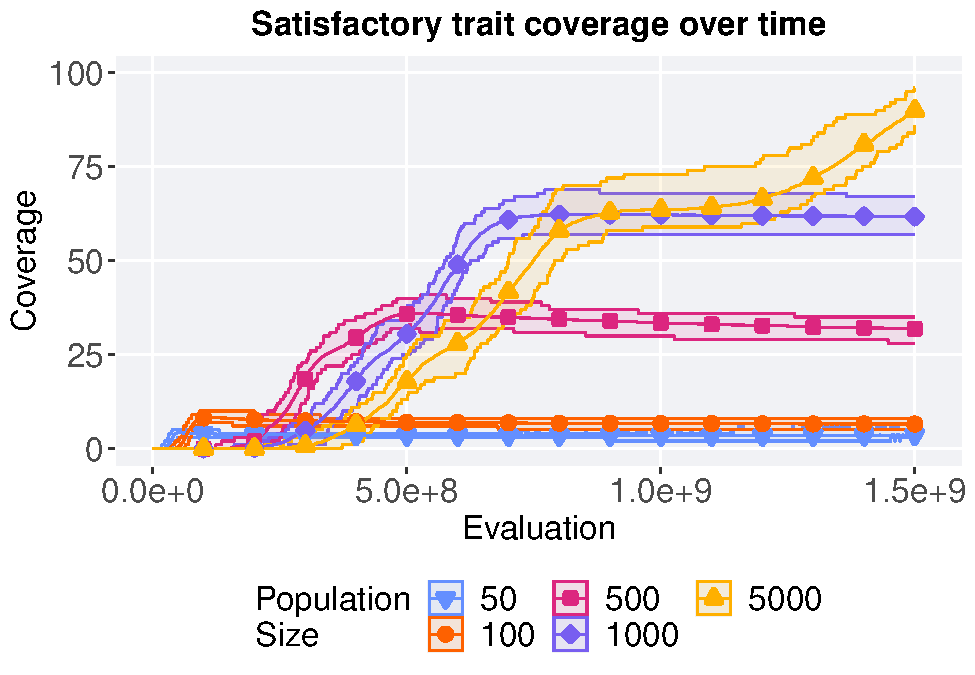
\includegraphics[width=1\linewidth]{lexicase-analysis-supplemental_files/figure-latex/con-200-sat-ot-1}

\hypertarget{best-satisfactory-trait-coverage-found-throughout-run-1}{%
\subsection{Best satisfactory trait coverage found throughout run}\label{best-satisfactory-trait-coverage-found-throughout-run-1}}

Satisfactory trait coverage of the best population found throughout an evolutionary run.

\begin{Shaded}
\begin{Highlighting}[]
\FunctionTok{ggplot}\NormalTok{(best, }\FunctionTok{aes}\NormalTok{(}\AttributeTok{x =}\NormalTok{ pop\_size, }\AttributeTok{y =}\NormalTok{ coverage, }\AttributeTok{color =}\NormalTok{ pop\_size, }\AttributeTok{fill =}\NormalTok{ pop\_size, }\AttributeTok{shape =}\NormalTok{ pop\_size)) }\SpecialCharTok{+}
  \FunctionTok{geom\_flat\_violin}\NormalTok{(}\AttributeTok{position =} \FunctionTok{position\_nudge}\NormalTok{(}\AttributeTok{x =}\NormalTok{ .}\DecValTok{1}\NormalTok{, }\AttributeTok{y =} \DecValTok{0}\NormalTok{), }\AttributeTok{scale =} \StringTok{\textquotesingle{}width\textquotesingle{}}\NormalTok{, }\AttributeTok{alpha =} \FloatTok{0.2}\NormalTok{, }\AttributeTok{width =} \FloatTok{1.5}\NormalTok{) }\SpecialCharTok{+}
  \FunctionTok{geom\_boxplot}\NormalTok{(}\AttributeTok{color =} \StringTok{\textquotesingle{}black\textquotesingle{}}\NormalTok{, }\AttributeTok{width =}\NormalTok{ .}\DecValTok{07}\NormalTok{, }\AttributeTok{outlier.shape =} \ConstantTok{NA}\NormalTok{, }\AttributeTok{alpha =} \FloatTok{0.0}\NormalTok{, }\AttributeTok{size =} \FloatTok{1.0}\NormalTok{, }\AttributeTok{position =} \FunctionTok{position\_nudge}\NormalTok{(}\AttributeTok{x =}\NormalTok{ .}\DecValTok{16}\NormalTok{, }\AttributeTok{y =} \DecValTok{0}\NormalTok{)) }\SpecialCharTok{+}
  \FunctionTok{geom\_point}\NormalTok{(}\AttributeTok{position =} \FunctionTok{position\_jitter}\NormalTok{(}\AttributeTok{width =} \FloatTok{0.02}\NormalTok{, }\AttributeTok{height =} \FloatTok{0.0001}\NormalTok{), }\AttributeTok{size =} \FloatTok{1.5}\NormalTok{, }\AttributeTok{alpha =} \FloatTok{1.0}\NormalTok{) }\SpecialCharTok{+}
  \FunctionTok{scale\_y\_continuous}\NormalTok{(}
    \AttributeTok{name=}\StringTok{"Coverage"}\NormalTok{,}
    \AttributeTok{limits=}\FunctionTok{c}\NormalTok{(}\DecValTok{0}\NormalTok{, }\DecValTok{100}\NormalTok{),}
    \AttributeTok{breaks=}\FunctionTok{seq}\NormalTok{(}\DecValTok{0}\NormalTok{,}\DecValTok{100}\NormalTok{, }\DecValTok{25}\NormalTok{),}
    \AttributeTok{labels=}\FunctionTok{c}\NormalTok{(}\StringTok{"0"}\NormalTok{, }\StringTok{"25"}\NormalTok{, }\StringTok{"50"}\NormalTok{, }\StringTok{"75"}\NormalTok{, }\StringTok{"100"}\NormalTok{),}
\NormalTok{  ) }\SpecialCharTok{+}
  \FunctionTok{scale\_x\_discrete}\NormalTok{(}
    \AttributeTok{name=}\StringTok{"Population Size"}
\NormalTok{  )}\SpecialCharTok{+}
  \FunctionTok{scale\_shape\_manual}\NormalTok{(}\AttributeTok{values=}\NormalTok{SHAPE)}\SpecialCharTok{+}
  \FunctionTok{scale\_colour\_manual}\NormalTok{(}\AttributeTok{values =}\NormalTok{ cb\_palette, ) }\SpecialCharTok{+}
  \FunctionTok{scale\_fill\_manual}\NormalTok{(}\AttributeTok{values =}\NormalTok{ cb\_palette) }\SpecialCharTok{+}
  \FunctionTok{ggtitle}\NormalTok{(}\StringTok{\textquotesingle{}Best satisfactory coverage\textquotesingle{}}\NormalTok{)}\SpecialCharTok{+}
\NormalTok{  p\_theme }\SpecialCharTok{+} \FunctionTok{coord\_flip}\NormalTok{() }\SpecialCharTok{+}
  \FunctionTok{guides}\NormalTok{(}
    \AttributeTok{shape=}\FunctionTok{guide\_legend}\NormalTok{(}\AttributeTok{nrow=}\DecValTok{2}\NormalTok{, }\AttributeTok{title.position =} \StringTok{"left"}\NormalTok{, }\AttributeTok{title =} \StringTok{\textquotesingle{}Population}\SpecialCharTok{\textbackslash{}n}\StringTok{Size\textquotesingle{}}\NormalTok{),}
    \AttributeTok{color=}\FunctionTok{guide\_legend}\NormalTok{(}\AttributeTok{nrow=}\DecValTok{2}\NormalTok{, }\AttributeTok{title.position =} \StringTok{"left"}\NormalTok{, }\AttributeTok{title =} \StringTok{\textquotesingle{}Population}\SpecialCharTok{\textbackslash{}n}\StringTok{Size\textquotesingle{}}\NormalTok{),}
    \AttributeTok{fill=}\FunctionTok{guide\_legend}\NormalTok{(}\AttributeTok{nrow=}\DecValTok{2}\NormalTok{, }\AttributeTok{title.position =} \StringTok{"left"}\NormalTok{, }\AttributeTok{title =} \StringTok{\textquotesingle{}Population}\SpecialCharTok{\textbackslash{}n}\StringTok{Size\textquotesingle{}}\NormalTok{)}
\NormalTok{  )}
\end{Highlighting}
\end{Shaded}

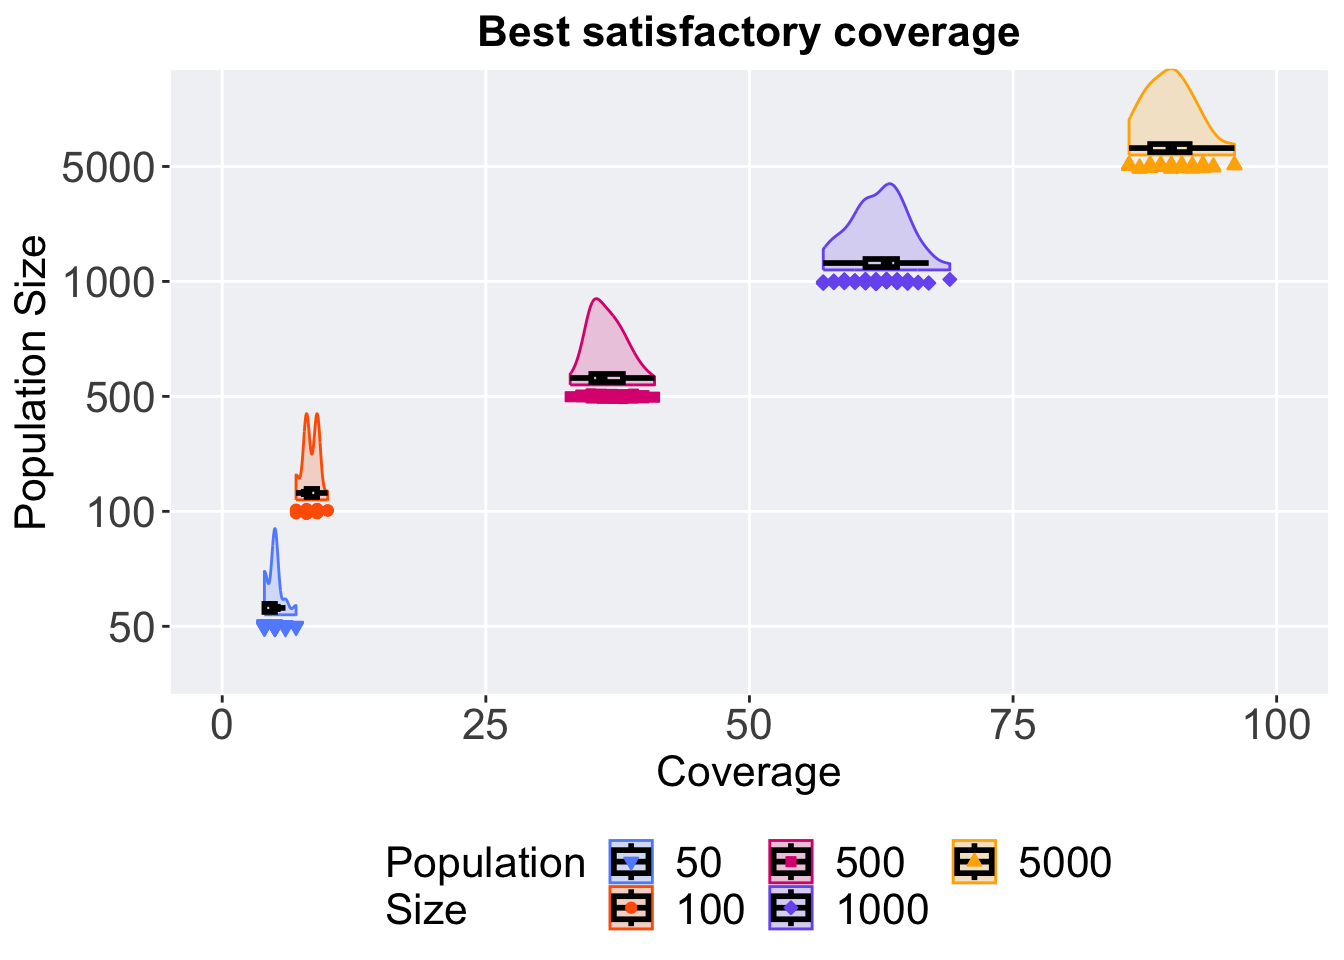
\includegraphics[width=1\linewidth]{lexicase-analysis-supplemental_files/figure-latex/con-200-sat-best-1}

\hypertarget{summary-statistics-3}{%
\subsubsection{Summary statistics}\label{summary-statistics-3}}

\begin{Shaded}
\begin{Highlighting}[]
\NormalTok{best }\SpecialCharTok{\%\textgreater{}\%}
  \FunctionTok{group\_by}\NormalTok{(pop\_size) }\SpecialCharTok{\%\textgreater{}\%}
\NormalTok{  dplyr}\SpecialCharTok{::}\FunctionTok{summarise}\NormalTok{(}
    \AttributeTok{count =} \FunctionTok{n}\NormalTok{(),}
    \AttributeTok{na\_cnt =} \FunctionTok{sum}\NormalTok{(}\FunctionTok{is.na}\NormalTok{(coverage)),}
    \AttributeTok{min =} \FunctionTok{min}\NormalTok{(coverage, }\AttributeTok{na.rm =} \ConstantTok{TRUE}\NormalTok{),}
    \AttributeTok{median =} \FunctionTok{median}\NormalTok{(coverage, }\AttributeTok{na.rm =} \ConstantTok{TRUE}\NormalTok{),}
    \AttributeTok{mean =} \FunctionTok{mean}\NormalTok{(coverage, }\AttributeTok{na.rm =} \ConstantTok{TRUE}\NormalTok{),}
    \AttributeTok{max =} \FunctionTok{max}\NormalTok{(coverage, }\AttributeTok{na.rm =} \ConstantTok{TRUE}\NormalTok{),}
    \AttributeTok{IQR =} \FunctionTok{IQR}\NormalTok{(coverage, }\AttributeTok{na.rm =} \ConstantTok{TRUE}\NormalTok{)}
\NormalTok{  )}
\end{Highlighting}
\end{Shaded}

\begin{verbatim}
## # A tibble: 5 x 8
##   pop_size count na_cnt   min median  mean   max   IQR
##   <fct>    <int>  <int> <int>  <dbl> <dbl> <int> <dbl>
## 1 50          50      0     4      5  4.94     7  1   
## 2 100         50      0     7      8  8.38    10  1   
## 3 500         50      0    33     36 36.5     41  3   
## 4 1000        50      0    57     63 62.3     69  3   
## 5 5000        50      0    86     90 90.0     96  3.75
\end{verbatim}

\hypertarget{kruskal-wallis-test-3}{%
\subsubsection{Kruskal-Wallis test}\label{kruskal-wallis-test-3}}

\begin{Shaded}
\begin{Highlighting}[]
\FunctionTok{kruskal.test}\NormalTok{(coverage }\SpecialCharTok{\textasciitilde{}}\NormalTok{ pop\_size, }\AttributeTok{data =}\NormalTok{ best)}
\end{Highlighting}
\end{Shaded}

\begin{verbatim}
## 
##  Kruskal-Wallis rank sum test
## 
## data:  coverage by pop_size
## Kruskal-Wallis chi-squared = 239.68, df = 4, p-value < 2.2e-16
\end{verbatim}

\hypertarget{pairwise-wilcoxon-test-3}{%
\subsubsection{Pairwise wilcoxon test}\label{pairwise-wilcoxon-test-3}}

\begin{Shaded}
\begin{Highlighting}[]
\FunctionTok{pairwise.wilcox.test}\NormalTok{(}\AttributeTok{x =}\NormalTok{ best}\SpecialCharTok{$}\NormalTok{coverage, }\AttributeTok{g =}\NormalTok{ best}\SpecialCharTok{$}\NormalTok{pop\_size, }\AttributeTok{p.adjust.method =} \StringTok{"bonferroni"}\NormalTok{,}
                     \AttributeTok{paired =} \ConstantTok{FALSE}\NormalTok{, }\AttributeTok{conf.int =} \ConstantTok{FALSE}\NormalTok{, }\AttributeTok{alternative =} \StringTok{\textquotesingle{}g\textquotesingle{}}\NormalTok{)}
\end{Highlighting}
\end{Shaded}

\begin{verbatim}
## 
##  Pairwise comparisons using Wilcoxon rank sum test with continuity correction 
## 
## data:  best$coverage and best$pop_size 
## 
##      50     100    500    1000  
## 100  <2e-16 -      -      -     
## 500  <2e-16 <2e-16 -      -     
## 1000 <2e-16 <2e-16 <2e-16 -     
## 5000 <2e-16 <2e-16 <2e-16 <2e-16
## 
## P value adjustment method: bonferroni
\end{verbatim}

\hypertarget{contradictory-objectives-300-results}{%
\chapter{Contradictory objectives 300 results}\label{contradictory-objectives-300-results}}

Here we report the \textbf{activation gene coverage} and \textbf{satisfactory trait coverage} was found on the contradictory objectives diagnostic.
50 replicates were conducted for each population size explored.
Activation gene coverage is calculated by finding all the unique activation genes found within a given population.
Satisfactory trait coverage is calculated by finding all the unique satisfactory traits found within a given population.

\hypertarget{analysis-setup-3}{%
\section{Analysis setup}\label{analysis-setup-3}}

\begin{Shaded}
\begin{Highlighting}[]
\FunctionTok{library}\NormalTok{(ggplot2)}
\FunctionTok{library}\NormalTok{(cowplot)}
\FunctionTok{library}\NormalTok{(dplyr)}
\FunctionTok{library}\NormalTok{(PupillometryR)}

\CommentTok{\# over time data}
\NormalTok{over\_time }\OtherTok{\textless{}{-}} \FunctionTok{read.csv}\NormalTok{(}\StringTok{"../Paper\_Data/Contradictory{-}300/ot.csv"}\NormalTok{, }\AttributeTok{header =} \ConstantTok{TRUE}\NormalTok{, }\AttributeTok{stringsAsFactors =} \ConstantTok{FALSE}\NormalTok{)}
\NormalTok{over\_time}\SpecialCharTok{$}\NormalTok{pop\_size }\OtherTok{\textless{}{-}} \FunctionTok{factor}\NormalTok{(over\_time}\SpecialCharTok{$}\NormalTok{pop\_size, }\AttributeTok{levels =}\NormalTok{ NAMES)}

\CommentTok{\# best performance data}
\NormalTok{best }\OtherTok{\textless{}{-}} \FunctionTok{read.csv}\NormalTok{(}\StringTok{\textquotesingle{}../Paper\_Data/Contradictory{-}300/best.csv\textquotesingle{}}\NormalTok{, }\AttributeTok{header =} \ConstantTok{TRUE}\NormalTok{, }\AttributeTok{stringsAsFactors =} \ConstantTok{FALSE}\NormalTok{)}
\NormalTok{best}\SpecialCharTok{$}\NormalTok{pop\_size }\OtherTok{\textless{}{-}} \FunctionTok{factor}\NormalTok{(best}\SpecialCharTok{$}\NormalTok{pop\_size, }\AttributeTok{levels =}\NormalTok{ NAMES)}
\end{Highlighting}
\end{Shaded}

\hypertarget{activation-gene-coverage-2}{%
\section{Activation gene coverage}\label{activation-gene-coverage-2}}

\hypertarget{coverage-over-time-4}{%
\subsection{Coverage over time}\label{coverage-over-time-4}}

Performance of the best solution in the population at each generation over time.

\begin{Shaded}
\begin{Highlighting}[]
\CommentTok{\# aggregate}
\NormalTok{lines }\OtherTok{=} \FunctionTok{filter}\NormalTok{(over\_time,eval }\SpecialCharTok{!=} \DecValTok{0}\NormalTok{) }\SpecialCharTok{\%\textgreater{}\%}
  \FunctionTok{group\_by}\NormalTok{(pop\_size, eval) }\SpecialCharTok{\%\textgreater{}\%}
\NormalTok{  dplyr}\SpecialCharTok{::}\FunctionTok{summarise}\NormalTok{(}
    \AttributeTok{min =} \FunctionTok{min}\NormalTok{(activation\_coverage),}
    \AttributeTok{mean =} \FunctionTok{mean}\NormalTok{(activation\_coverage),}
    \AttributeTok{max =} \FunctionTok{max}\NormalTok{(activation\_coverage)}
\NormalTok{  )}
\NormalTok{lines}\SpecialCharTok{$}\NormalTok{pop\_size }\OtherTok{\textless{}{-}} \FunctionTok{factor}\NormalTok{(lines}\SpecialCharTok{$}\NormalTok{pop\_size, }\AttributeTok{levels =}\NormalTok{ NAMES)}

\FunctionTok{ggplot}\NormalTok{(lines, }\FunctionTok{aes}\NormalTok{(}\AttributeTok{x=}\NormalTok{eval, }\AttributeTok{y=}\NormalTok{mean, }\AttributeTok{group =}\NormalTok{ pop\_size, }\AttributeTok{fill =}\NormalTok{ pop\_size, }\AttributeTok{color =}\NormalTok{ pop\_size, }\AttributeTok{shape =}\NormalTok{ pop\_size)) }\SpecialCharTok{+}
  \FunctionTok{geom\_ribbon}\NormalTok{(}\FunctionTok{aes}\NormalTok{(}\AttributeTok{ymin =}\NormalTok{ min, }\AttributeTok{ymax =}\NormalTok{ max), }\AttributeTok{alpha =} \FloatTok{0.1}\NormalTok{) }\SpecialCharTok{+}
  \FunctionTok{geom\_line}\NormalTok{(}\AttributeTok{linewidth =} \FloatTok{0.5}\NormalTok{) }\SpecialCharTok{+}
  \FunctionTok{geom\_point}\NormalTok{(}\AttributeTok{data =} \FunctionTok{filter}\NormalTok{(lines, eval }\SpecialCharTok{\%\%} \DecValTok{100000000} \SpecialCharTok{==} \DecValTok{0} \SpecialCharTok{\&}\NormalTok{ eval }\SpecialCharTok{!=} \DecValTok{0}\NormalTok{), }\AttributeTok{size =} \FloatTok{1.0}\NormalTok{, }\AttributeTok{stroke =} \FloatTok{2.0}\NormalTok{, }\AttributeTok{alpha =} \FloatTok{1.0}\NormalTok{) }\SpecialCharTok{+}
  \FunctionTok{scale\_y\_continuous}\NormalTok{(}
    \AttributeTok{name=}\StringTok{"Coverage"}\NormalTok{,}
    \AttributeTok{limits=}\FunctionTok{c}\NormalTok{(}\DecValTok{0}\NormalTok{, }\DecValTok{100}\NormalTok{),}
    \AttributeTok{breaks=}\FunctionTok{seq}\NormalTok{(}\DecValTok{0}\NormalTok{,}\DecValTok{100}\NormalTok{, }\DecValTok{25}\NormalTok{),}
    \AttributeTok{labels=}\FunctionTok{c}\NormalTok{(}\StringTok{"0"}\NormalTok{, }\StringTok{"25"}\NormalTok{, }\StringTok{"50"}\NormalTok{, }\StringTok{"75"}\NormalTok{, }\StringTok{"100"}\NormalTok{)}
\NormalTok{  ) }\SpecialCharTok{+}
  \FunctionTok{scale\_x\_continuous}\NormalTok{(}
    \AttributeTok{name=}\StringTok{"Evaluation"}\NormalTok{,}
    \AttributeTok{labels =} \FunctionTok{c}\NormalTok{(}\StringTok{\textquotesingle{}0.0e+0\textquotesingle{}}\NormalTok{, }\StringTok{\textquotesingle{}5.0e+8\textquotesingle{}}\NormalTok{,}\StringTok{\textquotesingle{}1.0e+9\textquotesingle{}}\NormalTok{,}\StringTok{\textquotesingle{}1.5e+9\textquotesingle{}}\NormalTok{),}
    \AttributeTok{limits =} \FunctionTok{c}\NormalTok{(}\DecValTok{0}\NormalTok{,}\DecValTok{1530000000}\NormalTok{)}

\NormalTok{  ) }\SpecialCharTok{+}
  \FunctionTok{scale\_shape\_manual}\NormalTok{(}\AttributeTok{values=}\NormalTok{SHAPE)}\SpecialCharTok{+}
  \FunctionTok{scale\_colour\_manual}\NormalTok{(}\AttributeTok{values =}\NormalTok{ cb\_palette) }\SpecialCharTok{+}
  \FunctionTok{scale\_fill\_manual}\NormalTok{(}\AttributeTok{values =}\NormalTok{ cb\_palette) }\SpecialCharTok{+}
  \FunctionTok{ggtitle}\NormalTok{(}\StringTok{\textquotesingle{}Activation gene coverage over time\textquotesingle{}}\NormalTok{)}\SpecialCharTok{+}
\NormalTok{  p\_theme }\SpecialCharTok{+}
  \FunctionTok{guides}\NormalTok{(}
    \AttributeTok{shape=}\FunctionTok{guide\_legend}\NormalTok{(}\AttributeTok{nrow=}\DecValTok{2}\NormalTok{, }\AttributeTok{title.position =} \StringTok{"left"}\NormalTok{, }\AttributeTok{title =} \StringTok{\textquotesingle{}Population}\SpecialCharTok{\textbackslash{}n}\StringTok{Size\textquotesingle{}}\NormalTok{),}
    \AttributeTok{color=}\FunctionTok{guide\_legend}\NormalTok{(}\AttributeTok{nrow=}\DecValTok{2}\NormalTok{, }\AttributeTok{title.position =} \StringTok{"left"}\NormalTok{, }\AttributeTok{title =} \StringTok{\textquotesingle{}Population}\SpecialCharTok{\textbackslash{}n}\StringTok{Size\textquotesingle{}}\NormalTok{),}
    \AttributeTok{fill=}\FunctionTok{guide\_legend}\NormalTok{(}\AttributeTok{nrow=}\DecValTok{2}\NormalTok{, }\AttributeTok{title.position =} \StringTok{"left"}\NormalTok{, }\AttributeTok{title =} \StringTok{\textquotesingle{}Population}\SpecialCharTok{\textbackslash{}n}\StringTok{Size\textquotesingle{}}\NormalTok{)}
\NormalTok{  )}
\end{Highlighting}
\end{Shaded}

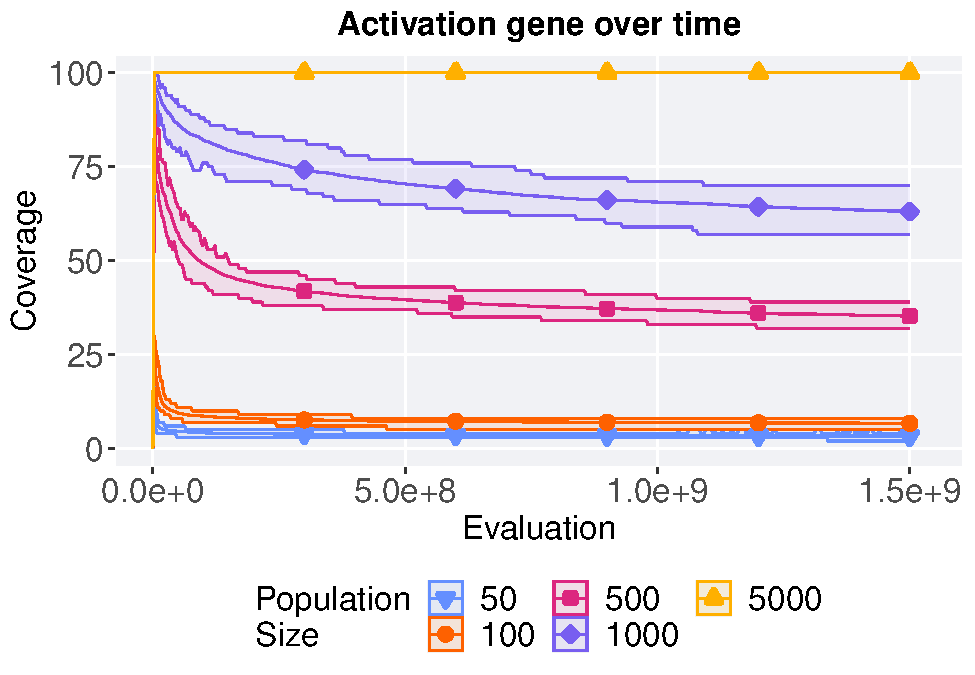
\includegraphics[width=1\linewidth]{lexicase-analysis-supplemental_files/figure-latex/con-300-act-ot-1}

\hypertarget{satisfactory-trait-coverage-2}{%
\section{Satisfactory trait coverage}\label{satisfactory-trait-coverage-2}}

\hypertarget{coverage-over-time-5}{%
\subsection{Coverage over time}\label{coverage-over-time-5}}

Satisfactory trait coverage over time.

\begin{Shaded}
\begin{Highlighting}[]
\CommentTok{\# aggregate}
\NormalTok{lines }\OtherTok{=}\NormalTok{ over\_time }\SpecialCharTok{\%\textgreater{}\%}
  \FunctionTok{group\_by}\NormalTok{(pop\_size, eval) }\SpecialCharTok{\%\textgreater{}\%}
\NormalTok{  dplyr}\SpecialCharTok{::}\FunctionTok{summarise}\NormalTok{(}
    \AttributeTok{min =} \FunctionTok{min}\NormalTok{(satisfactory\_coverage),}
    \AttributeTok{mean =} \FunctionTok{mean}\NormalTok{(satisfactory\_coverage),}
    \AttributeTok{max =} \FunctionTok{max}\NormalTok{(satisfactory\_coverage)}
\NormalTok{  )}
\NormalTok{lines}\SpecialCharTok{$}\NormalTok{pop\_size }\OtherTok{\textless{}{-}} \FunctionTok{factor}\NormalTok{(lines}\SpecialCharTok{$}\NormalTok{pop\_size, }\AttributeTok{levels =}\NormalTok{ NAMES)}

\FunctionTok{ggplot}\NormalTok{(lines, }\FunctionTok{aes}\NormalTok{(}\AttributeTok{x=}\NormalTok{eval, }\AttributeTok{y=}\NormalTok{mean, }\AttributeTok{group =}\NormalTok{ pop\_size, }\AttributeTok{fill =}\NormalTok{ pop\_size, }\AttributeTok{color =}\NormalTok{ pop\_size, }\AttributeTok{shape =}\NormalTok{ pop\_size)) }\SpecialCharTok{+}
  \FunctionTok{geom\_ribbon}\NormalTok{(}\FunctionTok{aes}\NormalTok{(}\AttributeTok{ymin =}\NormalTok{ min, }\AttributeTok{ymax =}\NormalTok{ max), }\AttributeTok{alpha =} \FloatTok{0.1}\NormalTok{) }\SpecialCharTok{+}
  \FunctionTok{geom\_line}\NormalTok{(}\AttributeTok{linewidth =} \FloatTok{0.5}\NormalTok{) }\SpecialCharTok{+}
  \FunctionTok{geom\_point}\NormalTok{(}\AttributeTok{data =} \FunctionTok{filter}\NormalTok{(lines, eval }\SpecialCharTok{\%\%} \DecValTok{100000000} \SpecialCharTok{==} \DecValTok{0} \SpecialCharTok{\&}\NormalTok{ eval }\SpecialCharTok{!=} \DecValTok{0}\NormalTok{), }\AttributeTok{size =} \FloatTok{1.0}\NormalTok{, }\AttributeTok{stroke =} \FloatTok{2.0}\NormalTok{, }\AttributeTok{alpha =} \FloatTok{1.0}\NormalTok{) }\SpecialCharTok{+}
  \FunctionTok{scale\_y\_continuous}\NormalTok{(}
    \AttributeTok{name=}\StringTok{"Coverage"}\NormalTok{,}
    \AttributeTok{limits=}\FunctionTok{c}\NormalTok{(}\DecValTok{0}\NormalTok{, }\DecValTok{75}\NormalTok{),}
    \AttributeTok{breaks=}\FunctionTok{seq}\NormalTok{(}\DecValTok{0}\NormalTok{,}\DecValTok{75}\NormalTok{, }\DecValTok{25}\NormalTok{),}
    \AttributeTok{labels=}\FunctionTok{c}\NormalTok{(}\StringTok{"0"}\NormalTok{, }\StringTok{"25"}\NormalTok{, }\StringTok{"50"}\NormalTok{, }\StringTok{"75"}\NormalTok{)}
\NormalTok{  ) }\SpecialCharTok{+}
  \FunctionTok{scale\_x\_continuous}\NormalTok{(}
    \AttributeTok{name=}\StringTok{"Evaluation"}\NormalTok{,}
    \AttributeTok{labels =} \FunctionTok{c}\NormalTok{(}\StringTok{\textquotesingle{}0.0e+0\textquotesingle{}}\NormalTok{, }\StringTok{\textquotesingle{}5.0e+8\textquotesingle{}}\NormalTok{,}\StringTok{\textquotesingle{}1.0e+9\textquotesingle{}}\NormalTok{,}\StringTok{\textquotesingle{}1.5e+9\textquotesingle{}}\NormalTok{),}
    \AttributeTok{limits =} \FunctionTok{c}\NormalTok{(}\DecValTok{0}\NormalTok{,}\DecValTok{1530000000}\NormalTok{)}

\NormalTok{  ) }\SpecialCharTok{+}
  \FunctionTok{scale\_shape\_manual}\NormalTok{(}\AttributeTok{values=}\NormalTok{SHAPE)}\SpecialCharTok{+}
  \FunctionTok{scale\_colour\_manual}\NormalTok{(}\AttributeTok{values =}\NormalTok{ cb\_palette) }\SpecialCharTok{+}
  \FunctionTok{scale\_fill\_manual}\NormalTok{(}\AttributeTok{values =}\NormalTok{ cb\_palette) }\SpecialCharTok{+}
  \FunctionTok{ggtitle}\NormalTok{(}\StringTok{\textquotesingle{}Satisfactory trait coverage over time\textquotesingle{}}\NormalTok{)}\SpecialCharTok{+}
\NormalTok{  p\_theme }\SpecialCharTok{+}
  \FunctionTok{guides}\NormalTok{(}
    \AttributeTok{shape=}\FunctionTok{guide\_legend}\NormalTok{(}\AttributeTok{nrow=}\DecValTok{2}\NormalTok{, }\AttributeTok{title.position =} \StringTok{"left"}\NormalTok{, }\AttributeTok{title =} \StringTok{\textquotesingle{}Population}\SpecialCharTok{\textbackslash{}n}\StringTok{Size\textquotesingle{}}\NormalTok{),}
    \AttributeTok{color=}\FunctionTok{guide\_legend}\NormalTok{(}\AttributeTok{nrow=}\DecValTok{2}\NormalTok{, }\AttributeTok{title.position =} \StringTok{"left"}\NormalTok{, }\AttributeTok{title =} \StringTok{\textquotesingle{}Population}\SpecialCharTok{\textbackslash{}n}\StringTok{Size\textquotesingle{}}\NormalTok{),}
    \AttributeTok{fill=}\FunctionTok{guide\_legend}\NormalTok{(}\AttributeTok{nrow=}\DecValTok{2}\NormalTok{, }\AttributeTok{title.position =} \StringTok{"left"}\NormalTok{, }\AttributeTok{title =} \StringTok{\textquotesingle{}Population}\SpecialCharTok{\textbackslash{}n}\StringTok{Size\textquotesingle{}}\NormalTok{)}
\NormalTok{  )}
\end{Highlighting}
\end{Shaded}

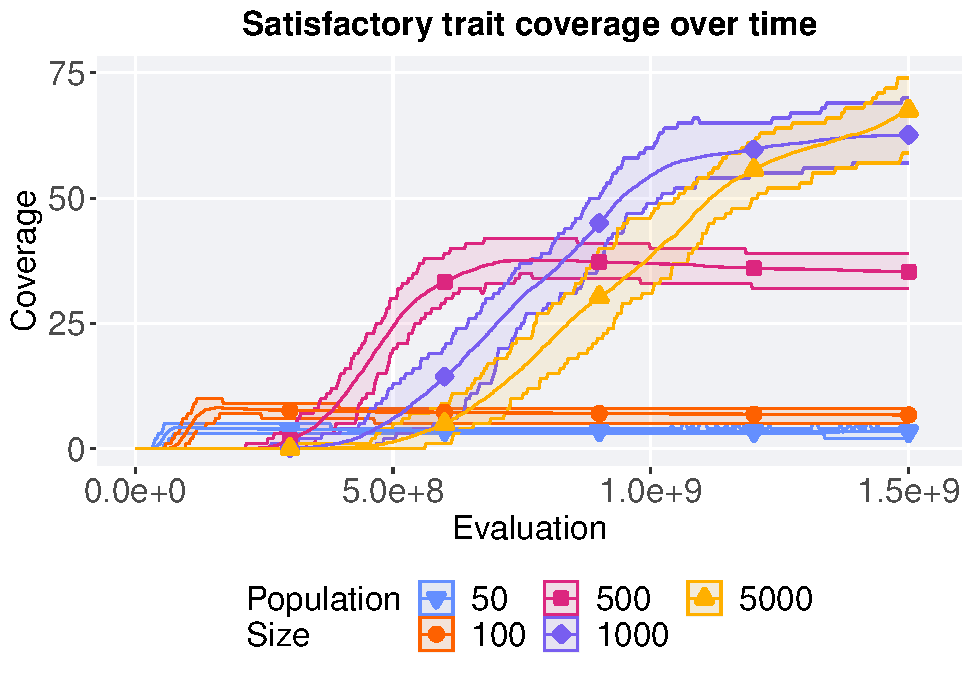
\includegraphics[width=1\linewidth]{lexicase-analysis-supplemental_files/figure-latex/con-300-sat-ot-1}

\hypertarget{best-satisfactory-trait-coverage-found-throughout-run-2}{%
\subsection{Best satisfactory trait coverage found throughout run}\label{best-satisfactory-trait-coverage-found-throughout-run-2}}

Satisfactory trait coverage of the best population found throughout an evolutionary run.

\begin{Shaded}
\begin{Highlighting}[]
\FunctionTok{ggplot}\NormalTok{(best, }\FunctionTok{aes}\NormalTok{(}\AttributeTok{x =}\NormalTok{ pop\_size, }\AttributeTok{y =}\NormalTok{ coverage, }\AttributeTok{color =}\NormalTok{ pop\_size, }\AttributeTok{fill =}\NormalTok{ pop\_size, }\AttributeTok{shape =}\NormalTok{ pop\_size)) }\SpecialCharTok{+}
  \FunctionTok{geom\_flat\_violin}\NormalTok{(}\AttributeTok{position =} \FunctionTok{position\_nudge}\NormalTok{(}\AttributeTok{x =}\NormalTok{ .}\DecValTok{1}\NormalTok{, }\AttributeTok{y =} \DecValTok{0}\NormalTok{), }\AttributeTok{scale =} \StringTok{\textquotesingle{}width\textquotesingle{}}\NormalTok{, }\AttributeTok{alpha =} \FloatTok{0.2}\NormalTok{, }\AttributeTok{width =} \FloatTok{1.5}\NormalTok{) }\SpecialCharTok{+}
  \FunctionTok{geom\_boxplot}\NormalTok{(}\AttributeTok{color =} \StringTok{\textquotesingle{}black\textquotesingle{}}\NormalTok{, }\AttributeTok{width =}\NormalTok{ .}\DecValTok{07}\NormalTok{, }\AttributeTok{outlier.shape =} \ConstantTok{NA}\NormalTok{, }\AttributeTok{alpha =} \FloatTok{0.0}\NormalTok{, }\AttributeTok{size =} \FloatTok{1.0}\NormalTok{, }\AttributeTok{position =} \FunctionTok{position\_nudge}\NormalTok{(}\AttributeTok{x =}\NormalTok{ .}\DecValTok{16}\NormalTok{, }\AttributeTok{y =} \DecValTok{0}\NormalTok{)) }\SpecialCharTok{+}
  \FunctionTok{geom\_point}\NormalTok{(}\AttributeTok{position =} \FunctionTok{position\_jitter}\NormalTok{(}\AttributeTok{width =} \FloatTok{0.02}\NormalTok{, }\AttributeTok{height =} \FloatTok{0.0001}\NormalTok{), }\AttributeTok{size =} \FloatTok{1.5}\NormalTok{, }\AttributeTok{alpha =} \FloatTok{1.0}\NormalTok{) }\SpecialCharTok{+}
  \FunctionTok{scale\_y\_continuous}\NormalTok{(}
    \AttributeTok{name=}\StringTok{"Coverage"}\NormalTok{,}
    \AttributeTok{limits=}\FunctionTok{c}\NormalTok{(}\DecValTok{0}\NormalTok{, }\DecValTok{75}\NormalTok{),}
    \AttributeTok{breaks=}\FunctionTok{seq}\NormalTok{(}\DecValTok{0}\NormalTok{,}\DecValTok{75}\NormalTok{, }\DecValTok{25}\NormalTok{),}
    \AttributeTok{labels=}\FunctionTok{c}\NormalTok{(}\StringTok{"0"}\NormalTok{, }\StringTok{"25"}\NormalTok{, }\StringTok{"50"}\NormalTok{, }\StringTok{"75"}\NormalTok{)}
\NormalTok{  ) }\SpecialCharTok{+}
  \FunctionTok{scale\_x\_discrete}\NormalTok{(}
    \AttributeTok{name=}\StringTok{"Population Size"}
\NormalTok{  )}\SpecialCharTok{+}
  \FunctionTok{scale\_shape\_manual}\NormalTok{(}\AttributeTok{values=}\NormalTok{SHAPE)}\SpecialCharTok{+}
  \FunctionTok{scale\_colour\_manual}\NormalTok{(}\AttributeTok{values =}\NormalTok{ cb\_palette, ) }\SpecialCharTok{+}
  \FunctionTok{scale\_fill\_manual}\NormalTok{(}\AttributeTok{values =}\NormalTok{ cb\_palette) }\SpecialCharTok{+}
  \FunctionTok{ggtitle}\NormalTok{(}\StringTok{\textquotesingle{}Best satisfactory coverage\textquotesingle{}}\NormalTok{)}\SpecialCharTok{+}
\NormalTok{  p\_theme }\SpecialCharTok{+} \FunctionTok{coord\_flip}\NormalTok{() }\SpecialCharTok{+}
  \FunctionTok{guides}\NormalTok{(}
    \AttributeTok{shape=}\FunctionTok{guide\_legend}\NormalTok{(}\AttributeTok{nrow=}\DecValTok{2}\NormalTok{, }\AttributeTok{title.position =} \StringTok{"left"}\NormalTok{, }\AttributeTok{title =} \StringTok{\textquotesingle{}Population}\SpecialCharTok{\textbackslash{}n}\StringTok{Size\textquotesingle{}}\NormalTok{),}
    \AttributeTok{color=}\FunctionTok{guide\_legend}\NormalTok{(}\AttributeTok{nrow=}\DecValTok{2}\NormalTok{, }\AttributeTok{title.position =} \StringTok{"left"}\NormalTok{, }\AttributeTok{title =} \StringTok{\textquotesingle{}Population}\SpecialCharTok{\textbackslash{}n}\StringTok{Size\textquotesingle{}}\NormalTok{),}
    \AttributeTok{fill=}\FunctionTok{guide\_legend}\NormalTok{(}\AttributeTok{nrow=}\DecValTok{2}\NormalTok{, }\AttributeTok{title.position =} \StringTok{"left"}\NormalTok{, }\AttributeTok{title =} \StringTok{\textquotesingle{}Population}\SpecialCharTok{\textbackslash{}n}\StringTok{Size\textquotesingle{}}\NormalTok{)}
\NormalTok{  )}
\end{Highlighting}
\end{Shaded}

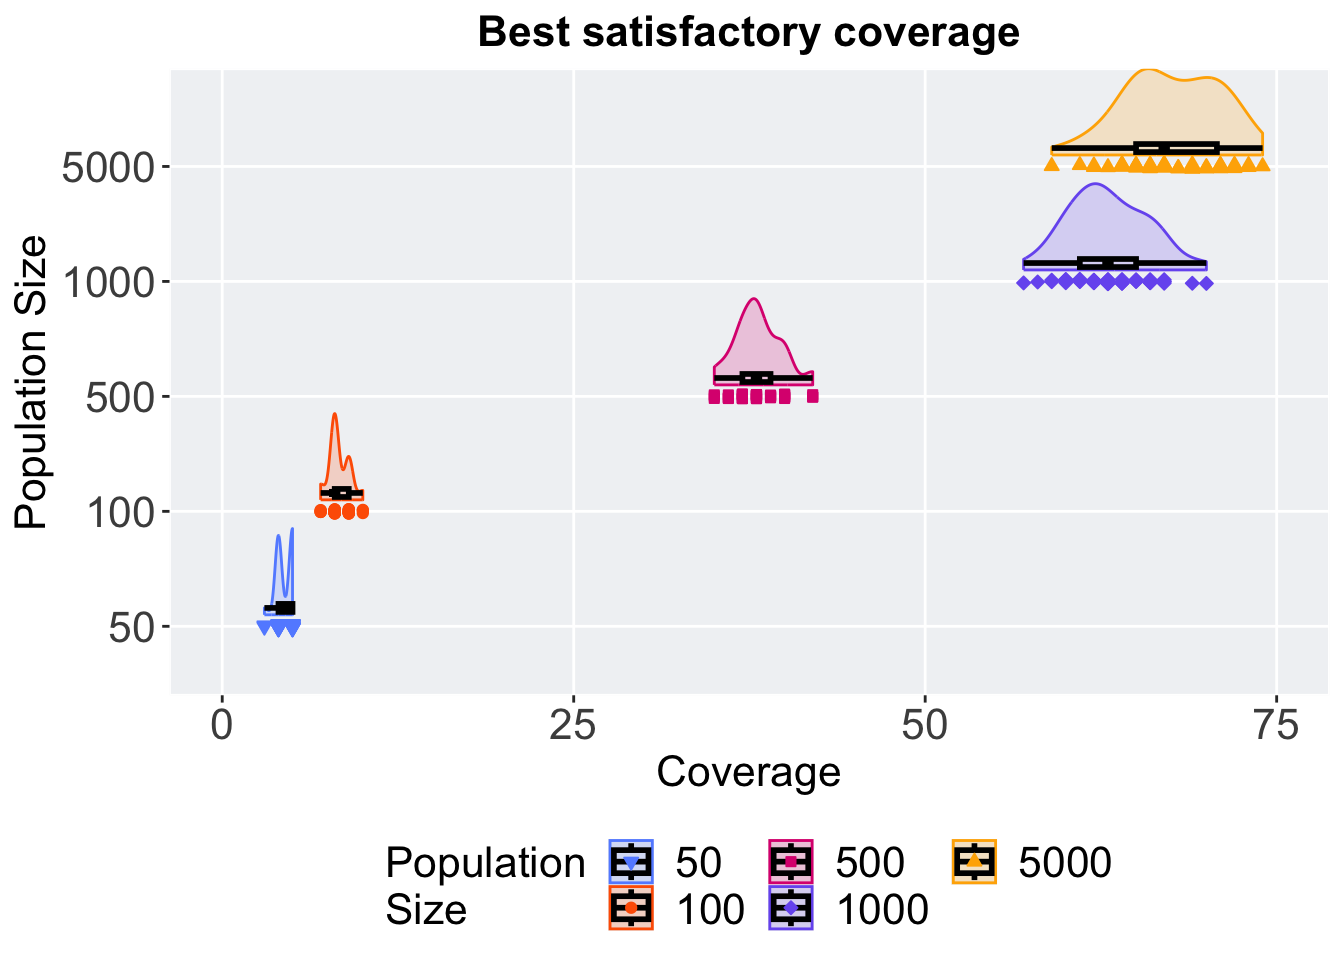
\includegraphics[width=1\linewidth]{lexicase-analysis-supplemental_files/figure-latex/con-300-sat-best-1}

\hypertarget{summary-statistics-4}{%
\subsubsection{Summary statistics}\label{summary-statistics-4}}

\begin{Shaded}
\begin{Highlighting}[]
\NormalTok{best }\SpecialCharTok{\%\textgreater{}\%}
  \FunctionTok{group\_by}\NormalTok{(pop\_size) }\SpecialCharTok{\%\textgreater{}\%}
\NormalTok{  dplyr}\SpecialCharTok{::}\FunctionTok{summarise}\NormalTok{(}
    \AttributeTok{count =} \FunctionTok{n}\NormalTok{(),}
    \AttributeTok{na\_cnt =} \FunctionTok{sum}\NormalTok{(}\FunctionTok{is.na}\NormalTok{(coverage)),}
    \AttributeTok{min =} \FunctionTok{min}\NormalTok{(coverage, }\AttributeTok{na.rm =} \ConstantTok{TRUE}\NormalTok{),}
    \AttributeTok{median =} \FunctionTok{median}\NormalTok{(coverage, }\AttributeTok{na.rm =} \ConstantTok{TRUE}\NormalTok{),}
    \AttributeTok{mean =} \FunctionTok{mean}\NormalTok{(coverage, }\AttributeTok{na.rm =} \ConstantTok{TRUE}\NormalTok{),}
    \AttributeTok{max =} \FunctionTok{max}\NormalTok{(coverage, }\AttributeTok{na.rm =} \ConstantTok{TRUE}\NormalTok{),}
    \AttributeTok{IQR =} \FunctionTok{IQR}\NormalTok{(coverage, }\AttributeTok{na.rm =} \ConstantTok{TRUE}\NormalTok{)}
\NormalTok{  )}
\end{Highlighting}
\end{Shaded}

\begin{verbatim}
## # A tibble: 5 x 8
##   pop_size count na_cnt   min median  mean   max   IQR
##   <fct>    <int>  <int> <int>  <dbl> <dbl> <int> <dbl>
## 1 50          50      0     3    4.5  4.46     5  1   
## 2 100         50      0     7    8    8.3     10  1   
## 3 500         50      0    35   38   38.1     42  2   
## 4 1000        50      0    57   63   63.0     70  4   
## 5 5000        50      0    59   67   67.5     74  5.75
\end{verbatim}

\hypertarget{kruskal-wallis-test-4}{%
\subsubsection{Kruskal-Wallis test}\label{kruskal-wallis-test-4}}

\begin{Shaded}
\begin{Highlighting}[]
\FunctionTok{kruskal.test}\NormalTok{(coverage }\SpecialCharTok{\textasciitilde{}}\NormalTok{ pop\_size, }\AttributeTok{data =}\NormalTok{ best)}
\end{Highlighting}
\end{Shaded}

\begin{verbatim}
## 
##  Kruskal-Wallis rank sum test
## 
## data:  coverage by pop_size
## Kruskal-Wallis chi-squared = 233.56, df = 4, p-value < 2.2e-16
\end{verbatim}

\hypertarget{pairwise-wilcoxon-test-4}{%
\subsubsection{Pairwise wilcoxon test}\label{pairwise-wilcoxon-test-4}}

\begin{Shaded}
\begin{Highlighting}[]
\FunctionTok{pairwise.wilcox.test}\NormalTok{(}\AttributeTok{x =}\NormalTok{ best}\SpecialCharTok{$}\NormalTok{coverage, }\AttributeTok{g =}\NormalTok{ best}\SpecialCharTok{$}\NormalTok{pop\_size, }\AttributeTok{p.adjust.method =} \StringTok{"bonferroni"}\NormalTok{,}
                     \AttributeTok{paired =} \ConstantTok{FALSE}\NormalTok{, }\AttributeTok{conf.int =} \ConstantTok{FALSE}\NormalTok{, }\AttributeTok{alternative =} \StringTok{\textquotesingle{}g\textquotesingle{}}\NormalTok{)}
\end{Highlighting}
\end{Shaded}

\begin{verbatim}
## 
##  Pairwise comparisons using Wilcoxon rank sum test with continuity correction 
## 
## data:  best$coverage and best$pop_size 
## 
##      50      100     500     1000   
## 100  < 2e-16 -       -       -      
## 500  < 2e-16 < 2e-16 -       -      
## 1000 < 2e-16 < 2e-16 < 2e-16 -      
## 5000 < 2e-16 < 2e-16 < 2e-16 2.3e-08
## 
## P value adjustment method: bonferroni
\end{verbatim}

\hypertarget{contradictory-objectives-500-results}{%
\chapter{Contradictory objectives 500 results}\label{contradictory-objectives-500-results}}

Here we report the \textbf{activation gene coverage} and \textbf{satisfactory trait coverage} was found on the contradictory objectives diagnostic.
50 replicates were conducted for each population size explored.
Activation gene coverage is calculated by finding all the unique activation genes found within a given population.
Satisfactory trait coverage is calculated by finding all the unique satisfactory traits found within a given population.

\hypertarget{analysis-setup-4}{%
\section{Analysis setup}\label{analysis-setup-4}}

\begin{Shaded}
\begin{Highlighting}[]
\FunctionTok{library}\NormalTok{(ggplot2)}
\FunctionTok{library}\NormalTok{(cowplot)}
\FunctionTok{library}\NormalTok{(dplyr)}
\FunctionTok{library}\NormalTok{(PupillometryR)}

\CommentTok{\# over time data}
\NormalTok{over\_time }\OtherTok{\textless{}{-}} \FunctionTok{read.csv}\NormalTok{(}\StringTok{"../Paper\_Data/Contradictory{-}500/ot.csv"}\NormalTok{, }\AttributeTok{header =} \ConstantTok{TRUE}\NormalTok{, }\AttributeTok{stringsAsFactors =} \ConstantTok{FALSE}\NormalTok{)}
\NormalTok{over\_time}\SpecialCharTok{$}\NormalTok{pop\_size }\OtherTok{\textless{}{-}} \FunctionTok{factor}\NormalTok{(over\_time}\SpecialCharTok{$}\NormalTok{pop\_size, }\AttributeTok{levels =}\NormalTok{ NAMES)}

\CommentTok{\# best performance data}
\NormalTok{best }\OtherTok{\textless{}{-}} \FunctionTok{read.csv}\NormalTok{(}\StringTok{\textquotesingle{}../Paper\_Data/Contradictory{-}500/best.csv\textquotesingle{}}\NormalTok{, }\AttributeTok{header =} \ConstantTok{TRUE}\NormalTok{, }\AttributeTok{stringsAsFactors =} \ConstantTok{FALSE}\NormalTok{)}
\NormalTok{best}\SpecialCharTok{$}\NormalTok{pop\_size }\OtherTok{\textless{}{-}} \FunctionTok{factor}\NormalTok{(best}\SpecialCharTok{$}\NormalTok{pop\_size, }\AttributeTok{levels =}\NormalTok{ NAMES)}
\end{Highlighting}
\end{Shaded}

\hypertarget{activation-gene-coverage-3}{%
\section{Activation gene coverage}\label{activation-gene-coverage-3}}

\hypertarget{coverage-over-time-6}{%
\subsection{Coverage over time}\label{coverage-over-time-6}}

Performance of the best solution in the population at each generation over time.

\begin{Shaded}
\begin{Highlighting}[]
\NormalTok{lines }\OtherTok{=} \FunctionTok{filter}\NormalTok{(over\_time,eval }\SpecialCharTok{!=} \DecValTok{0}\NormalTok{) }\SpecialCharTok{\%\textgreater{}\%}
  \FunctionTok{group\_by}\NormalTok{(pop\_size, eval) }\SpecialCharTok{\%\textgreater{}\%}
\NormalTok{  dplyr}\SpecialCharTok{::}\FunctionTok{summarise}\NormalTok{(}
    \AttributeTok{min =} \FunctionTok{min}\NormalTok{(activation\_coverage),}
    \AttributeTok{mean =} \FunctionTok{mean}\NormalTok{(activation\_coverage),}
    \AttributeTok{max =} \FunctionTok{max}\NormalTok{(activation\_coverage)}
\NormalTok{  )}
\NormalTok{lines}\SpecialCharTok{$}\NormalTok{pop\_size }\OtherTok{\textless{}{-}} \FunctionTok{factor}\NormalTok{(lines}\SpecialCharTok{$}\NormalTok{pop\_size, }\AttributeTok{levels =}\NormalTok{ NAMES)}

\FunctionTok{ggplot}\NormalTok{(lines, }\FunctionTok{aes}\NormalTok{(}\AttributeTok{x=}\NormalTok{eval, }\AttributeTok{y=}\NormalTok{mean, }\AttributeTok{group =}\NormalTok{ pop\_size, }\AttributeTok{fill =}\NormalTok{ pop\_size, }\AttributeTok{color =}\NormalTok{ pop\_size, }\AttributeTok{shape =}\NormalTok{ pop\_size)) }\SpecialCharTok{+}
  \FunctionTok{geom\_ribbon}\NormalTok{(}\FunctionTok{aes}\NormalTok{(}\AttributeTok{ymin =}\NormalTok{ min, }\AttributeTok{ymax =}\NormalTok{ max), }\AttributeTok{alpha =} \FloatTok{0.1}\NormalTok{) }\SpecialCharTok{+}
  \FunctionTok{geom\_line}\NormalTok{(}\AttributeTok{linewidth =} \FloatTok{0.5}\NormalTok{) }\SpecialCharTok{+}
  \FunctionTok{geom\_point}\NormalTok{(}\AttributeTok{data =} \FunctionTok{filter}\NormalTok{(lines, eval }\SpecialCharTok{\%\%} \DecValTok{100000000} \SpecialCharTok{==} \DecValTok{0} \SpecialCharTok{\&}\NormalTok{ eval }\SpecialCharTok{!=} \DecValTok{0}\NormalTok{), }\AttributeTok{size =} \FloatTok{1.0}\NormalTok{, }\AttributeTok{stroke =} \FloatTok{2.0}\NormalTok{, }\AttributeTok{alpha =} \FloatTok{1.0}\NormalTok{) }\SpecialCharTok{+}
  \FunctionTok{scale\_y\_continuous}\NormalTok{(}
    \AttributeTok{name=}\StringTok{"Coverage"}\NormalTok{,}
    \AttributeTok{limits=}\FunctionTok{c}\NormalTok{(}\DecValTok{0}\NormalTok{, }\DecValTok{100}\NormalTok{),}
    \AttributeTok{breaks=}\FunctionTok{seq}\NormalTok{(}\DecValTok{0}\NormalTok{,}\DecValTok{100}\NormalTok{, }\DecValTok{25}\NormalTok{),}
    \AttributeTok{labels=}\FunctionTok{c}\NormalTok{(}\StringTok{"0"}\NormalTok{, }\StringTok{"25"}\NormalTok{, }\StringTok{"50"}\NormalTok{, }\StringTok{"75"}\NormalTok{, }\StringTok{"100"}\NormalTok{)}
\NormalTok{  ) }\SpecialCharTok{+}
  \FunctionTok{scale\_x\_continuous}\NormalTok{(}
    \AttributeTok{name=}\StringTok{"Evaluation"}\NormalTok{,}
    \AttributeTok{labels =} \FunctionTok{c}\NormalTok{(}\StringTok{\textquotesingle{}0.0e+0\textquotesingle{}}\NormalTok{, }\StringTok{\textquotesingle{}5.0e+8\textquotesingle{}}\NormalTok{,}\StringTok{\textquotesingle{}1.0e+9\textquotesingle{}}\NormalTok{,}\StringTok{\textquotesingle{}1.5e+9\textquotesingle{}}\NormalTok{),}
    \AttributeTok{limits =} \FunctionTok{c}\NormalTok{(}\DecValTok{0}\NormalTok{,}\DecValTok{1520000000}\NormalTok{)}

\NormalTok{  ) }\SpecialCharTok{+}
  \FunctionTok{scale\_shape\_manual}\NormalTok{(}\AttributeTok{values=}\NormalTok{SHAPE)}\SpecialCharTok{+}
  \FunctionTok{scale\_colour\_manual}\NormalTok{(}\AttributeTok{values =}\NormalTok{ cb\_palette) }\SpecialCharTok{+}
  \FunctionTok{scale\_fill\_manual}\NormalTok{(}\AttributeTok{values =}\NormalTok{ cb\_palette) }\SpecialCharTok{+}
  \FunctionTok{ggtitle}\NormalTok{(}\StringTok{\textquotesingle{}Activation gene coverage over time\textquotesingle{}}\NormalTok{)}\SpecialCharTok{+}
\NormalTok{  p\_theme }\SpecialCharTok{+}
  \FunctionTok{guides}\NormalTok{(}
    \AttributeTok{shape=}\FunctionTok{guide\_legend}\NormalTok{(}\AttributeTok{nrow=}\DecValTok{2}\NormalTok{, }\AttributeTok{title.position =} \StringTok{"left"}\NormalTok{, }\AttributeTok{title =} \StringTok{\textquotesingle{}Population}\SpecialCharTok{\textbackslash{}n}\StringTok{Size\textquotesingle{}}\NormalTok{),}
    \AttributeTok{color=}\FunctionTok{guide\_legend}\NormalTok{(}\AttributeTok{nrow=}\DecValTok{2}\NormalTok{, }\AttributeTok{title.position =} \StringTok{"left"}\NormalTok{, }\AttributeTok{title =} \StringTok{\textquotesingle{}Population}\SpecialCharTok{\textbackslash{}n}\StringTok{Size\textquotesingle{}}\NormalTok{),}
    \AttributeTok{fill=}\FunctionTok{guide\_legend}\NormalTok{(}\AttributeTok{nrow=}\DecValTok{2}\NormalTok{, }\AttributeTok{title.position =} \StringTok{"left"}\NormalTok{, }\AttributeTok{title =} \StringTok{\textquotesingle{}Population}\SpecialCharTok{\textbackslash{}n}\StringTok{Size\textquotesingle{}}\NormalTok{)}
\NormalTok{  )}
\end{Highlighting}
\end{Shaded}

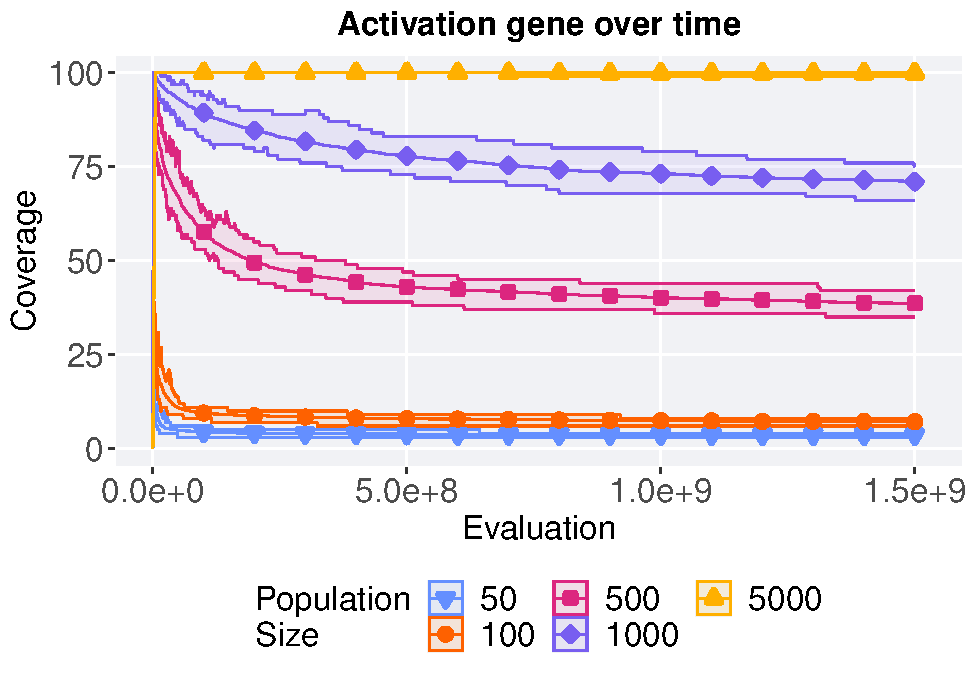
\includegraphics[width=1\linewidth]{lexicase-analysis-supplemental_files/figure-latex/con-500-act-ot-1}

\hypertarget{satisfactory-trait-coverage-3}{%
\section{Satisfactory trait coverage}\label{satisfactory-trait-coverage-3}}

\hypertarget{coverage-over-time-7}{%
\subsection{Coverage over time}\label{coverage-over-time-7}}

Satisfactory trait coverage over time.

\begin{Shaded}
\begin{Highlighting}[]
\CommentTok{\# aggregate}
\NormalTok{lines }\OtherTok{=}\NormalTok{ over\_time }\SpecialCharTok{\%\textgreater{}\%}
  \FunctionTok{group\_by}\NormalTok{(pop\_size, eval) }\SpecialCharTok{\%\textgreater{}\%}
\NormalTok{  dplyr}\SpecialCharTok{::}\FunctionTok{summarise}\NormalTok{(}
    \AttributeTok{min =} \FunctionTok{min}\NormalTok{(satisfactory\_coverage),}
    \AttributeTok{mean =} \FunctionTok{mean}\NormalTok{(satisfactory\_coverage),}
    \AttributeTok{max =} \FunctionTok{max}\NormalTok{(satisfactory\_coverage)}
\NormalTok{  )}
\NormalTok{lines}\SpecialCharTok{$}\NormalTok{pop\_size }\OtherTok{\textless{}{-}} \FunctionTok{factor}\NormalTok{(lines}\SpecialCharTok{$}\NormalTok{pop\_size, }\AttributeTok{levels =}\NormalTok{ NAMES)}

\FunctionTok{ggplot}\NormalTok{(lines, }\FunctionTok{aes}\NormalTok{(}\AttributeTok{x=}\NormalTok{eval, }\AttributeTok{y=}\NormalTok{mean, }\AttributeTok{group =}\NormalTok{ pop\_size, }\AttributeTok{fill =}\NormalTok{ pop\_size, }\AttributeTok{color =}\NormalTok{ pop\_size, }\AttributeTok{shape =}\NormalTok{ pop\_size)) }\SpecialCharTok{+}
  \FunctionTok{geom\_ribbon}\NormalTok{(}\FunctionTok{aes}\NormalTok{(}\AttributeTok{ymin =}\NormalTok{ min, }\AttributeTok{ymax =}\NormalTok{ max), }\AttributeTok{alpha =} \FloatTok{0.1}\NormalTok{) }\SpecialCharTok{+}
  \FunctionTok{geom\_line}\NormalTok{(}\AttributeTok{linewidth =} \FloatTok{0.5}\NormalTok{) }\SpecialCharTok{+}
  \FunctionTok{geom\_point}\NormalTok{(}\AttributeTok{data =} \FunctionTok{filter}\NormalTok{(lines, eval }\SpecialCharTok{\%\%} \DecValTok{100000000} \SpecialCharTok{==} \DecValTok{0} \SpecialCharTok{\&}\NormalTok{ eval }\SpecialCharTok{!=} \DecValTok{0}\NormalTok{), }\AttributeTok{size =} \FloatTok{1.0}\NormalTok{, }\AttributeTok{stroke =} \FloatTok{2.0}\NormalTok{, }\AttributeTok{alpha =} \FloatTok{1.0}\NormalTok{) }\SpecialCharTok{+}
  \FunctionTok{scale\_y\_continuous}\NormalTok{(}
    \AttributeTok{name=}\StringTok{"Coverage"}\NormalTok{,}
    \AttributeTok{limits=}\FunctionTok{c}\NormalTok{(}\DecValTok{0}\NormalTok{, }\DecValTok{60}\NormalTok{),}
    \AttributeTok{breaks=}\FunctionTok{seq}\NormalTok{(}\DecValTok{0}\NormalTok{,}\DecValTok{60}\NormalTok{, }\DecValTok{15}\NormalTok{),}
    \AttributeTok{labels=}\FunctionTok{c}\NormalTok{(}\StringTok{"0"}\NormalTok{, }\StringTok{"15"}\NormalTok{, }\StringTok{"30"}\NormalTok{, }\StringTok{"45"}\NormalTok{, }\StringTok{"60"}\NormalTok{)}
\NormalTok{  ) }\SpecialCharTok{+}
  \FunctionTok{scale\_x\_continuous}\NormalTok{(}
    \AttributeTok{name=}\StringTok{"Evaluation"}\NormalTok{,}
    \AttributeTok{labels =} \FunctionTok{c}\NormalTok{(}\StringTok{\textquotesingle{}0.0e+0\textquotesingle{}}\NormalTok{, }\StringTok{\textquotesingle{}5.0e+8\textquotesingle{}}\NormalTok{,}\StringTok{\textquotesingle{}1.0e+9\textquotesingle{}}\NormalTok{,}\StringTok{\textquotesingle{}1.5e+9\textquotesingle{}}\NormalTok{),}
    \AttributeTok{limits =} \FunctionTok{c}\NormalTok{(}\DecValTok{0}\NormalTok{,}\DecValTok{1520000000}\NormalTok{)}

\NormalTok{  ) }\SpecialCharTok{+}
  \FunctionTok{scale\_shape\_manual}\NormalTok{(}\AttributeTok{values=}\NormalTok{SHAPE)}\SpecialCharTok{+}
  \FunctionTok{scale\_colour\_manual}\NormalTok{(}\AttributeTok{values =}\NormalTok{ cb\_palette) }\SpecialCharTok{+}
  \FunctionTok{scale\_fill\_manual}\NormalTok{(}\AttributeTok{values =}\NormalTok{ cb\_palette) }\SpecialCharTok{+}
  \FunctionTok{ggtitle}\NormalTok{(}\StringTok{\textquotesingle{}Satisfactory trait coverage over time\textquotesingle{}}\NormalTok{)}\SpecialCharTok{+}
\NormalTok{  p\_theme }\SpecialCharTok{+}
  \FunctionTok{guides}\NormalTok{(}
    \AttributeTok{shape=}\FunctionTok{guide\_legend}\NormalTok{(}\AttributeTok{nrow=}\DecValTok{2}\NormalTok{, }\AttributeTok{title.position =} \StringTok{"left"}\NormalTok{, }\AttributeTok{title =} \StringTok{\textquotesingle{}Population}\SpecialCharTok{\textbackslash{}n}\StringTok{Size\textquotesingle{}}\NormalTok{),}
    \AttributeTok{color=}\FunctionTok{guide\_legend}\NormalTok{(}\AttributeTok{nrow=}\DecValTok{2}\NormalTok{, }\AttributeTok{title.position =} \StringTok{"left"}\NormalTok{, }\AttributeTok{title =} \StringTok{\textquotesingle{}Population}\SpecialCharTok{\textbackslash{}n}\StringTok{Size\textquotesingle{}}\NormalTok{),}
    \AttributeTok{fill=}\FunctionTok{guide\_legend}\NormalTok{(}\AttributeTok{nrow=}\DecValTok{2}\NormalTok{, }\AttributeTok{title.position =} \StringTok{"left"}\NormalTok{, }\AttributeTok{title =} \StringTok{\textquotesingle{}Population}\SpecialCharTok{\textbackslash{}n}\StringTok{Size\textquotesingle{}}\NormalTok{)}
\NormalTok{  )}
\end{Highlighting}
\end{Shaded}

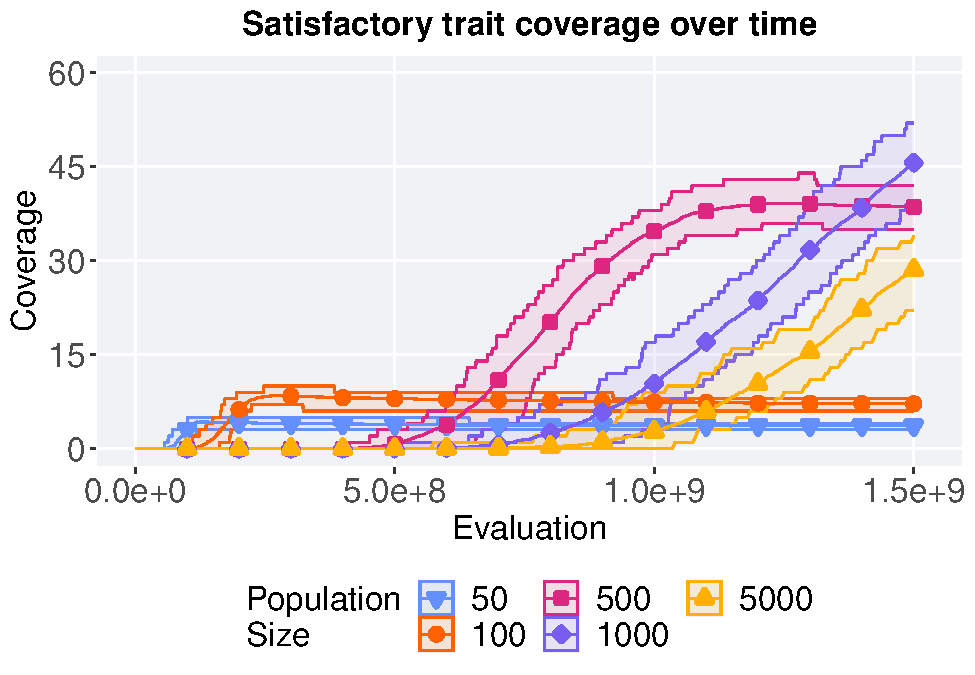
\includegraphics[width=1\linewidth]{lexicase-analysis-supplemental_files/figure-latex/con-500-sat-ot-1}

\hypertarget{best-satisfactory-trait-coverage-found-throughout-run-3}{%
\subsection{Best satisfactory trait coverage found throughout run}\label{best-satisfactory-trait-coverage-found-throughout-run-3}}

Satisfactory trait coverage of the best population found throughout an evolutionary run.

\begin{Shaded}
\begin{Highlighting}[]
\FunctionTok{ggplot}\NormalTok{(best, }\FunctionTok{aes}\NormalTok{(}\AttributeTok{x =}\NormalTok{ pop\_size, }\AttributeTok{y =}\NormalTok{ coverage, }\AttributeTok{color =}\NormalTok{ pop\_size, }\AttributeTok{fill =}\NormalTok{ pop\_size, }\AttributeTok{shape =}\NormalTok{ pop\_size)) }\SpecialCharTok{+}
  \FunctionTok{geom\_flat\_violin}\NormalTok{(}\AttributeTok{position =} \FunctionTok{position\_nudge}\NormalTok{(}\AttributeTok{x =}\NormalTok{ .}\DecValTok{1}\NormalTok{, }\AttributeTok{y =} \DecValTok{0}\NormalTok{), }\AttributeTok{scale =} \StringTok{\textquotesingle{}width\textquotesingle{}}\NormalTok{, }\AttributeTok{alpha =} \FloatTok{0.2}\NormalTok{, }\AttributeTok{width =} \FloatTok{1.5}\NormalTok{) }\SpecialCharTok{+}
  \FunctionTok{geom\_boxplot}\NormalTok{(}\AttributeTok{color =} \StringTok{\textquotesingle{}black\textquotesingle{}}\NormalTok{, }\AttributeTok{width =}\NormalTok{ .}\DecValTok{07}\NormalTok{, }\AttributeTok{outlier.shape =} \ConstantTok{NA}\NormalTok{, }\AttributeTok{alpha =} \FloatTok{0.0}\NormalTok{, }\AttributeTok{size =} \FloatTok{1.0}\NormalTok{, }\AttributeTok{position =} \FunctionTok{position\_nudge}\NormalTok{(}\AttributeTok{x =}\NormalTok{ .}\DecValTok{16}\NormalTok{, }\AttributeTok{y =} \DecValTok{0}\NormalTok{)) }\SpecialCharTok{+}
  \FunctionTok{geom\_point}\NormalTok{(}\AttributeTok{position =} \FunctionTok{position\_jitter}\NormalTok{(}\AttributeTok{width =} \FloatTok{0.02}\NormalTok{, }\AttributeTok{height =} \FloatTok{0.0001}\NormalTok{), }\AttributeTok{size =} \FloatTok{1.5}\NormalTok{, }\AttributeTok{alpha =} \FloatTok{1.0}\NormalTok{) }\SpecialCharTok{+}
  \FunctionTok{scale\_y\_continuous}\NormalTok{(}
    \AttributeTok{name=}\StringTok{"Coverage"}\NormalTok{,}
    \AttributeTok{limits=}\FunctionTok{c}\NormalTok{(}\DecValTok{0}\NormalTok{, }\DecValTok{60}\NormalTok{),}
    \AttributeTok{breaks=}\FunctionTok{seq}\NormalTok{(}\DecValTok{0}\NormalTok{,}\DecValTok{60}\NormalTok{, }\DecValTok{15}\NormalTok{),}
    \AttributeTok{labels=}\FunctionTok{c}\NormalTok{(}\StringTok{"0"}\NormalTok{, }\StringTok{"15"}\NormalTok{, }\StringTok{"30"}\NormalTok{, }\StringTok{"45"}\NormalTok{, }\StringTok{"60"}\NormalTok{)}
\NormalTok{  ) }\SpecialCharTok{+}
  \FunctionTok{scale\_x\_discrete}\NormalTok{(}
    \AttributeTok{name=}\StringTok{"Population Size"}
\NormalTok{  )}\SpecialCharTok{+}
  \FunctionTok{scale\_shape\_manual}\NormalTok{(}\AttributeTok{values=}\NormalTok{SHAPE)}\SpecialCharTok{+}
  \FunctionTok{scale\_colour\_manual}\NormalTok{(}\AttributeTok{values =}\NormalTok{ cb\_palette, ) }\SpecialCharTok{+}
  \FunctionTok{scale\_fill\_manual}\NormalTok{(}\AttributeTok{values =}\NormalTok{ cb\_palette) }\SpecialCharTok{+}
  \FunctionTok{ggtitle}\NormalTok{(}\StringTok{\textquotesingle{}Best satisfactory coverage\textquotesingle{}}\NormalTok{)}\SpecialCharTok{+}
\NormalTok{  p\_theme }\SpecialCharTok{+} \FunctionTok{coord\_flip}\NormalTok{() }\SpecialCharTok{+}
  \FunctionTok{guides}\NormalTok{(}
    \AttributeTok{shape=}\FunctionTok{guide\_legend}\NormalTok{(}\AttributeTok{nrow=}\DecValTok{2}\NormalTok{, }\AttributeTok{title.position =} \StringTok{"left"}\NormalTok{, }\AttributeTok{title =} \StringTok{\textquotesingle{}Population}\SpecialCharTok{\textbackslash{}n}\StringTok{Size\textquotesingle{}}\NormalTok{),}
    \AttributeTok{color=}\FunctionTok{guide\_legend}\NormalTok{(}\AttributeTok{nrow=}\DecValTok{2}\NormalTok{, }\AttributeTok{title.position =} \StringTok{"left"}\NormalTok{, }\AttributeTok{title =} \StringTok{\textquotesingle{}Population}\SpecialCharTok{\textbackslash{}n}\StringTok{Size\textquotesingle{}}\NormalTok{),}
    \AttributeTok{fill=}\FunctionTok{guide\_legend}\NormalTok{(}\AttributeTok{nrow=}\DecValTok{2}\NormalTok{, }\AttributeTok{title.position =} \StringTok{"left"}\NormalTok{, }\AttributeTok{title =} \StringTok{\textquotesingle{}Population}\SpecialCharTok{\textbackslash{}n}\StringTok{Size\textquotesingle{}}\NormalTok{)}
\NormalTok{  )}
\end{Highlighting}
\end{Shaded}

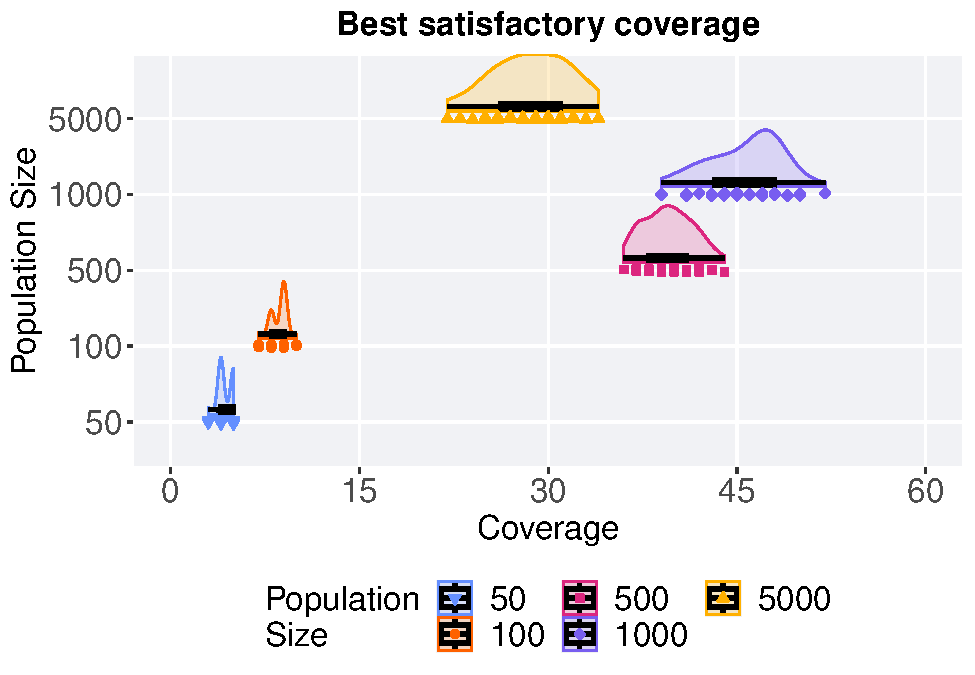
\includegraphics[width=1\linewidth]{lexicase-analysis-supplemental_files/figure-latex/con-500-sat-best-1}

\hypertarget{summary-statistics-5}{%
\subsubsection{Summary statistics}\label{summary-statistics-5}}

\begin{Shaded}
\begin{Highlighting}[]
\NormalTok{best }\SpecialCharTok{\%\textgreater{}\%}
  \FunctionTok{group\_by}\NormalTok{(pop\_size) }\SpecialCharTok{\%\textgreater{}\%}
\NormalTok{  dplyr}\SpecialCharTok{::}\FunctionTok{summarise}\NormalTok{(}
    \AttributeTok{count =} \FunctionTok{n}\NormalTok{(),}
    \AttributeTok{na\_cnt =} \FunctionTok{sum}\NormalTok{(}\FunctionTok{is.na}\NormalTok{(coverage)),}
    \AttributeTok{min =} \FunctionTok{min}\NormalTok{(coverage, }\AttributeTok{na.rm =} \ConstantTok{TRUE}\NormalTok{),}
    \AttributeTok{median =} \FunctionTok{median}\NormalTok{(coverage, }\AttributeTok{na.rm =} \ConstantTok{TRUE}\NormalTok{),}
    \AttributeTok{mean =} \FunctionTok{mean}\NormalTok{(coverage, }\AttributeTok{na.rm =} \ConstantTok{TRUE}\NormalTok{),}
    \AttributeTok{max =} \FunctionTok{max}\NormalTok{(coverage, }\AttributeTok{na.rm =} \ConstantTok{TRUE}\NormalTok{),}
    \AttributeTok{IQR =} \FunctionTok{IQR}\NormalTok{(coverage, }\AttributeTok{na.rm =} \ConstantTok{TRUE}\NormalTok{)}
\NormalTok{  )}
\end{Highlighting}
\end{Shaded}

\begin{verbatim}
## # A tibble: 5 x 8
##   pop_size count na_cnt   min median  mean   max   IQR
##   <fct>    <int>  <int> <int>  <dbl> <dbl> <int> <dbl>
## 1 50          50      0     3    4    4.36     5  1   
## 2 100         50      0     7    9    8.62    10  1   
## 3 500         50      0    36   39.5 39.6     44  3   
## 4 1000        50      0    39   46.5 45.7     52  4.75
## 5 5000        50      0    22   29   28.6     34  4.75
\end{verbatim}

\hypertarget{kruskal-wallis-test-5}{%
\subsubsection{Kruskal-Wallis test}\label{kruskal-wallis-test-5}}

\begin{Shaded}
\begin{Highlighting}[]
\FunctionTok{kruskal.test}\NormalTok{(coverage }\SpecialCharTok{\textasciitilde{}}\NormalTok{ pop\_size, }\AttributeTok{data =}\NormalTok{ best)}
\end{Highlighting}
\end{Shaded}

\begin{verbatim}
## 
##  Kruskal-Wallis rank sum test
## 
## data:  coverage by pop_size
## Kruskal-Wallis chi-squared = 237.63, df = 4, p-value < 2.2e-16
\end{verbatim}

\hypertarget{pairwise-wilcoxon-test-5}{%
\subsubsection{Pairwise wilcoxon test}\label{pairwise-wilcoxon-test-5}}

\begin{Shaded}
\begin{Highlighting}[]
\NormalTok{best}\SpecialCharTok{$}\NormalTok{pop\_size }\OtherTok{\textless{}{-}} \FunctionTok{factor}\NormalTok{(best}\SpecialCharTok{$}\NormalTok{pop\_size, }\AttributeTok{levels =} \FunctionTok{c}\NormalTok{(}\DecValTok{1000}\NormalTok{,}\DecValTok{500}\NormalTok{,}\DecValTok{5000}\NormalTok{,}\DecValTok{100}\NormalTok{,}\DecValTok{50}\NormalTok{))}
\FunctionTok{pairwise.wilcox.test}\NormalTok{(}\AttributeTok{x =}\NormalTok{ best}\SpecialCharTok{$}\NormalTok{coverage, }\AttributeTok{g =}\NormalTok{ best}\SpecialCharTok{$}\NormalTok{pop\_size, }\AttributeTok{p.adjust.method =} \StringTok{"bonferroni"}\NormalTok{,}
                     \AttributeTok{paired =} \ConstantTok{FALSE}\NormalTok{, }\AttributeTok{conf.int =} \ConstantTok{FALSE}\NormalTok{, }\AttributeTok{alternative =} \StringTok{\textquotesingle{}l\textquotesingle{}}\NormalTok{)}
\end{Highlighting}
\end{Shaded}

\begin{verbatim}
## 
##  Pairwise comparisons using Wilcoxon rank sum test with continuity correction 
## 
## data:  best$coverage and best$pop_size 
## 
##      1000    500     5000    100    
## 500  5.7e-14 -       -       -      
## 5000 < 2e-16 < 2e-16 -       -      
## 100  < 2e-16 < 2e-16 < 2e-16 -      
## 50   < 2e-16 < 2e-16 < 2e-16 < 2e-16
## 
## P value adjustment method: bonferroni
\end{verbatim}

  \bibliography{packages.bib,supplemental.bib}

\end{document}
